
\documentclass[10pt, a4paper, twoside]{report} % twoside => para distinguir paginas pares de impares

\usepackage[utf8]{inputenc} % codificacion
\usepackage[T1]{fontenc} % para acentos, copy and paste de documentos pdf...
\usepackage[spanish, english]{babel} % permite escribir acentos directamente sin \'
\decimalpoint % cambia la coma por el punto como separador de decimales en math mode

%%%%%%%%%%%%%%%%%%%%%%%%%%%%%%%%%%%%%%%%%%%%%%%%%%%%%%%%%%%%%%%%%%%%

\usepackage{makeidx} % para el indice de palabras
\makeindex

%%%%%%%%%%%%%%%%%%%%%%%%%%%%%%%%%%%%%%%%%%%%%%%%%%%%%%%%%%%%%%%%%%%%

\usepackage{multirow}

%%%%%%%%%%%%%%%%%%%%%%%%%%%%%%%%%%%%%%%%%%%%%%%%%%%%%%%%%%%%%%%%%%%%

\usepackage[usenames, dvipsnames]{xcolor} % usenames y dvipsnames permite usar los colores predefinidos
\definecolor{gray97}{gray}{.97}
%\definecolor{gray75}{gray}{.75}
\definecolor{gray45}{gray}{.45}

%%%%%%%%%%%%%%%%%%%%%%%%%%%%%%%%%%%%%%%%%%%%%%%%%%%%%%%%%%%%%%%%%%%%

\usepackage{amssymb} %para ciertos simbolos matemáticos
\usepackage{dsfont}
\newtheorem{theorem}{Teorema}[section] %definicion de teoremas
\usepackage{amsmath} % para el \text (en modo matematico)

%%%%%%%%%%%%%%%%%%%%%%%%%%%%%%%%%%%%%%%%%%%%%%%%%%%%%%%%%%%%%%%%%%%%

\usepackage{listings} % para la inclusion de codigo fuente de lenguajes de programacion
\renewcommand{\lstlistingname}{Listado} % para cambiar caption Listing por Listado
\renewcommand*{\lstlistlistingname}{Índice de listados} % para cambiar Lisitngs por Indice de Listados
\usepackage{etoolbox}
\newtoggle{InString}{} % monitorizar si estamos dentro de un string
\togglefalse{InString} % Inicialmente asumimos que no estamos en un string
\newcommand*{\ColorIfNotInString}[1]{\iftoggle{InString}{#1}{\color{red}#1}}%
\newcommand*{\ProcessQuote}[1]{#1\iftoggle{InString}{\global\togglefalse{InString}}{\global\toggletrue{InString}}}

\lstset{literate=%
    %{"}{{{\ProcessQuote{"}}}}1 % no coloreamos si estamos dentro de comillas dobles
    %{'}{{{\ProcessQuote{'}}}}1 % no coloreamos si estamos dentro de comillas simples
    {0}{{{\ColorIfNotInString{0}}}}1
    {1}{{{\ColorIfNotInString{1}}}}1
    {2}{{{\ColorIfNotInString{2}}}}1
    {3}{{{\ColorIfNotInString{3}}}}1
    {4}{{{\ColorIfNotInString{4}}}}1
    {5}{{{\ColorIfNotInString{5}}}}1
    {6}{{{\ColorIfNotInString{6}}}}1
    {7}{{{\ColorIfNotInString{7}}}}1
    {8}{{{\ColorIfNotInString{8}}}}1
    {9}{{{\ColorIfNotInString{9}}}}1
}

\lstset
  {
  backgroundcolor=\color{gray97},   % Indica el color de fondo
  basicstyle=\footnotesize,         % Fija el tamaño del tipo de letra utilizado para el código
  breakatwhitespace=false,          % Activarlo para que los saltos automáticos solo se apliquen en los espacios en blanco
  breaklines=true,                  % Activa el salto de línea automático
  captionpos=b,                     % Establece la posición de la leyenda del cuadro de código
  commentstyle=\color{gray45},      % Estilo de los comentarios
  deletekeywords={...},             % Si se quiere eliminar palabras clave del lenguaje
  escapeinside={\%*}{*)},           % Si quieres incorporar LaTeX dentro del propio código
  %escapeinside={\textbackslash}{*)},           % Si quieres incorporar LaTeX dentro del propio código
  frame=shadowbox,	                % Añade un marco al código
  keepspaces=true,                  % Mantiene los espacios en el texto (identacion) (puede necesitar columns=flexible).
  keywordstyle=\color{blue}\bfseries, % estilo de las palabras clave
  language=Python,                  % El lenguaje del código
  otherkeywords={*,..., yield,True,False,self}, % Si se quieren añadir otras palabras clave al lenguaje
  numbers=left,                     % Posición de los números de línea (none, left, right).
  numbersep=5pt,                    % Distancia de los números de línea al código
  numberstyle=\small\color{gray45}, % Estilo para los números de línea
  rulecolor=\color{black},          % Si no se activa, el color del marco puede cambiar en los saltos de línea entre textos
  showspaces=false,                 % Si se activa, muestra los espacios con guiones bajos
  showstringspaces=false,           % subraya solamente los espacios que estén en una cadena de esto
  showtabs=false,                   % muestra las tabulaciones que existan en cadenas de texto con guión bajo
  stepnumber=2,                     % Muestra solamente los números de línea que corresponden a cada salto. 
  stringstyle=\ttfamily\color{green}, % Estilo de las cadenas de texto
  tabsize=2,	                    % Establece el salto de las tabulaciones a 2 espacios
  title=\lstname ,                  % muestra el nombre de los ficheros incluidos al utilizar
  }
   
% minimizar fragmentado de listados
\lstnewenvironment{listing}[1][]
   {\lstset{#1}\pagebreak[0]}{\pagebreak[0]}

% estilo consola linux
%\lstdefinestyle{consola}
%   {
%   language=bash,
%   %basicstyle=\scriptsize\bf\ttfamily,
%   basicstyle=\footnotesize\bf\ttfamily,
%   %basicstyle=\small\bf\ttfamily,
%   backgroundcolor=\color{gray75},
%   escapeinside={\%*}{*)},
%   }
 
%%%%%%%%%%%%%%%%%%%%%%%%%%%%%%%%%%%%%%%%%%%%%%%%%%%%%%%%%%%%%%%%%%%%%%%%%%

\usepackage{graphicx} % para la inclusión de imagenes en el documento
\graphicspath{{C:/Users/David/Desktop/TFG/TFGLatex/imagenes}}

%%%%%%%%%%%%%%%%%%%%%%%%%%%%%%%%%%%%%%%%%%%%%%%%%%%%%%%%%%%%%%%%%%%%%%%%%%

\usepackage{wrapfig} % usado en la licencia

%%%%%%%%%%%%%%%%%%%%%%%%%%%%%%%%%%%%%%%%%%%%%%%%%%%%%%%%%%%%%%%%%%%%%%%%%%

\usepackage{framed} % para crear boxes

%%%%%%%%%%%%%%%%%%%%%%%%%%%%%%%%%%%%%%%%%%%%%%%%%%%%%%%%%%%%%%%%%%%%%%%%%%

%\usepackage{caption} % para quitar el prefijo de Figure:

%%%%%%%%%%%%%%%%%%%%%%%%%%%%%%%%%%%%%%%%%%%%%%%%%%%%%%%%%%%%%%%%%%%%%%%%%%

\usepackage[a4paper, top=2cm, bottom=2.25cm, outer=2.75cm, inner=2.75cm, 
heightrounded, marginparwidth=2.5cm, marginparsep=0.3cm]{geometry}  % estilo de pagina
%includehead,includefoot,

\usepackage{fancyhdr} % encabezados y pie de paginas

% clear default layout
\fancyhead{}
\fancyfoot{}

\fancyhead[LE,RO]{\textsc{\leftmark}} % muestra el nombre del capitulo en la cabecera
%\fancyhead[LE,RO]{\textsc{\rightmark}} % muestra el nombre de la seccion en la cabecera

\fancyfoot[C]{David Retana Ribeiro}
\fancyfoot[RE]{\thepage}
\fancyfoot[LO]{\thepage}

\renewcommand{\footrulewidth}{0.4pt}
\renewcommand{\headrulewidth}{0.4pt}
\pagestyle{fancy}

\fancypagestyle{plain}
  { % redefinimos plain porque se usa por defecto en las paginas de inicio de capitulo
  \fancyfoot[RE]{\thepage}
  \fancyfoot[LO]{\thepage}
  }

%%%%%%%%%%%%%%%%%%%%%%%%%%%%%%%%%%%%%%%%%%%%%%%%%%%%%%%%%%%%%%%%%%%%%%%%%

\setcounter{secnumdepth}{3} %para que en el indice de contenidos enumere hasta las subsubsecciones

%%%%%%%%%%%%%%%%%%%%%%%%%%%%%%%%%%%%%%%%%%%%%%%%%%%%%%%%%%%%%%%%%%%%%%%%%

\usepackage[hidelinks]{hyperref} %para las referencias cruzadas
\hypersetup
  {
  colorlinks,
  %linkcolor={violet!50!black},
  linkcolor=Brown, % link dentro del documento
  %linkcolor=red,
  citecolor={blue!50!black},
  urlcolor={blue!80!black}, % links de urls
  pdfstartview={FitH},    % fits the width of the page to the window
  pdftitle={Estudio comparativo de algoritmos paralelos de machine learning e implementación en Hadoop}, % title
  pdfauthor={David Retana Ribeiro}, % author  
  pdfsubject={Big data y machine learning},   % subject of the document
  pdfkeywords={computacion paralela, apache hadoop, apache spark, machine Learning, big data, python, k means,
               linear regression, naive bayes, yarn, hdfs, cluster, regresion lineal, deep learning}
  }
%%%%%%%%%%%%%%%%%%%%%%%%%%%%%%%%%%%%%%%%%%%%%%%%%%%%%%%%%%%%%%%%%%%%%%%%%

\begin{document}
\selectlanguage{spanish}

%%%%%%%%%%%%%%%%%%%%%%%%%%%%%%%%%%%%%%%%%%%%%%%%%%%%%%%%%%%%%%%%%%
%%%%%%%%%%%%%%%%%%%%%%%%%%% PORTADA %%%%%%%%%%%%%%%%%%%%%%%%%%%%%%
%%%%%%%%%%%%%%%%%%%%%%%%%%%%%%%%%%%%%%%%%%%%%%%%%%%%%%%%%%%%%%%%%%


\begin{titlepage}
  \begin{center}
    \vspace*{1cm}
    \Huge
    \textbf{UNIVERSIDAD COMPLUTENSE DE MADRID}\\
    \vspace{0.8cm}
    \LARGE

    \textbf{Facultad de Ciencias Matemáticas}\\
    \vspace{0.5cm}
    \vspace{0.5cm} 
    
\includegraphics[width=4cm]{C:/Users/David/Desktop/TFG/TFGLatex/imagenes/logoucm2.jpg} \\

    Trabajo Fin de Grado\\
    Especialidad: Ciencias de la computación\\
    \vspace{0.8cm}
    \Huge
    \textbf{Estudio comparativo de algoritmos}\\
    \textbf{paralelos de machine learning}\\
    \textbf{e implementación en Hadoop}\\
    \vfill
    \LARGE
    \vspace{1cm}
    \textbf{David Retana Ribeiro}\\
    \vspace{0.5cm}
    Tutor: Carlos Gregorio Rodríguez\\
    \vspace{0.5cm}
    \Large
    21 de Septiembre de 2017 
  \end{center}
\end{titlepage}



%%%%%%%%%%%%%%%%%%%%%%%%%%%%%%%%%%%%%%%%%%%%%%%%%%%%%%%%%%%%%%%%%%
%%%%%%%%%%%%%%%%%%%%%% PÁGINA EN BLANCO %%%%%%%%%%%%%%%%%%%%%%%%%%
%%%%%%%%%%%%%%%%%%%%%%%%%%%%%%%%%%%%%%%%%%%%%%%%%%%%%%%%%%%%%%%%%%

\newpage
%$\ $
\thispagestyle{empty} % para que no se enumere esta pagina y no tenga header ni footer
\null\vfill
%\noindent

%%%%%%%%%%%%%%%%%%%%%%%%%%%%%%%%%%%%%%%%%%%%%%%%%%%%%%%%%%%%%%%%%%
%%%%%%%%%%%%%%%%%%%%%%%%%%%% LICENCIA %%%%%%%%%%%%%%%%%%%%%%%%%%%%
%%%%%%%%%%%%%%%%%%%%%%%%%%%%%%%%%%%%%%%%%%%%%%%%%%%%%%%%%%%%%%%%%%

\newpage
%$\ $
\thispagestyle{empty} % para que no se enumere esta pagina
\null\vfill
%\noindent

%\pagenumbering{roman}

\textcopyright \hspace{0.3cm} Copyright $2017$ David Retana Ribeiro\\

\begin{wrapfigure}{r}{0.4\textwidth}
  \centering \url{https://creativecommons.org/licenses/by-sa/3.0/es/}
  \href{https://creativecommons.org/licenses/by-sa/3.0/es/}
       {
\includegraphics[width=0.3\textwidth]{C:/Users/David/Desktop/TFG/TFGLatex/imagenes/cc-by-sa.png}}
  %\caption*{\url{https://creativecommons.org/licenses/by-sa/3.0/es/}}
\end{wrapfigure}
\noindent Las imágenes contenidas en este documento \\
así como el código fuente y la información \\
que recoge, se encuentran licenciadas \\
bajo una licencia \textit{Creative Commons}.

\clearpage

%%%%%%%%%%%%%%%%%%%%%%%%%%%%%%%%%%%%%%%%%%%%%%%%%%%%%%%%%%%%%%%%%%
%%%%%%%%%%%%%%%%%%%%%%%%% DEDICATORIAS %%%%%%%%%%%%%%%%%%%%%%%%%%%
%%%%%%%%%%%%%%%%%%%%%%%%%%%%%%%%%%%%%%%%%%%%%%%%%%%%%%%%%%%%%%%%%%
\thispagestyle{empty}
\pagenumbering{roman} % si dejamos este en vez de el de arriba hay que revisar el \setcounter
\begin{flushright}
  \textit{Dedicado a: \\
  Mis padres, Rosa y Pedro, por ese apoyo incondicional a lo largo de toda mi vida \\
  Mis hermanos, Fátima y Carlos, por estar siempre ahí\\
  A mi tutor Carlos Gregorio por dirigirme en este trabajo\\
  A todos mis compañeros de CoreNetworks}
\end{flushright}

\newpage

%%%%%%%%%%%%%%%%%%%%%%%%%%%%%%%%%%%%%%%%%%%%%%%%%%%%%%%%%%%%%%%%%%
%%%%%%%%%%%%%%%% SOBRE EL AUTOR Y CONVENCIONES %%%%%%%%%%%%%%%%%%%
%%%%%%%%%%%%%%%%%%%%%%%%%%%%%%%%%%%%%%%%%%%%%%%%%%%%%%%%%%%%%%%%%%


\begin{table}
  \centering \textbf{\textsc{Sobre el autor}} % texto cabecera
  
  \begin{tabular}[t]{crl} % tabla
    \multirow{4}{*}{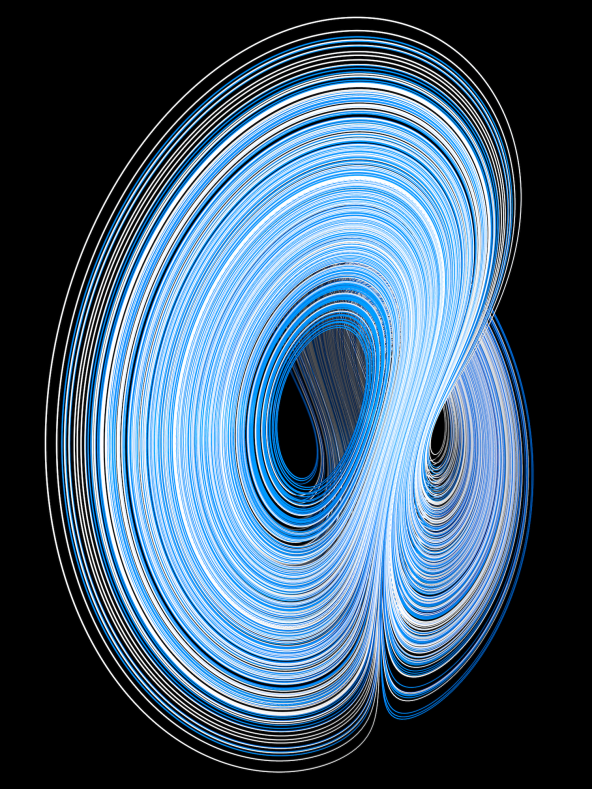
\includegraphics[scale=0.05]{C:/Users/David/Desktop/TFG/TFGLatex/imagenes/lorenz.png}} & \textsf{Nombre} & David Retana Ribeiro \\
                            & \textsf{Titulación} & Grado en Matemáticas \\
                            & \multirow{2}{*}{\textsf{correos}} & \texttt{davidretanaribeiro@gmail.com} \\
                            &                          & \texttt{dr4293@outlook.com} \\
    \textsf{LinkedIn} & \multicolumn{2}{l}{\url{https://www.linkedin.com/in/david-retana-ribeiro-519a56147/}} \\
    \textsf{GitHub}   & \multicolumn{2}{l}{\url{https://github.com/davidRetana}} \\
    \textsf{Kaggle}   & \multicolumn{2}{l}{\url{https://www.kaggle.com/davidretana}} \\
  \end{tabular}
  \label{sobre_el_autor} % etiqueta
\end{table}

\vspace*{1cm}

\noindent \textbf{Convenciones en la escritura del documento}:
\begin{itemize}
  \item Se usará \textit{letra en cursiva} para designar aquellos términos en inglés que no son 
        traducidos al español, como por ejemplo \textit{machine learning}, \textit{cluster}...\\
        También se usará para designar nombres propios como \textit{Creative Commons} o \textit{Apache}.
  \item La letra en \textbf{negrita} quedará reservada para hacer hincapié en ciertos términos que 
        quieran ser remarcados bien sea porque son importantes para el desarrollo del capítulo 
        o porque en ellos se base la idea a explicar en el capítulo.
  \item Las notas al pie de página se usan para explicar conceptos de manera breve y concisa, 
        así como evitar confusiones en la utilización de términos ambiguos.
  \item En numerosas ocasiones aparecerá ejemplos de códigos fuente y comandos de \textit{shell}, 
        éstos aparecerán destacados en un recuadro. Para los comandos \textit{UNIX}, los argumentos encerrados 
        entre signos de desigualdad (< >) indicarán parámetros a completar por el usuario mientras que 
        si están encerrados por corchetes ([ ]) indica que son opcionales.
  \item El código fuente escrito en \textit{Python} seguirá el estilo marcado por 
        \href{https://www.python.org/dev/peps/pep-0008/}{PEP8}.
  \item En el \autoref{chap:implementacion_paralela}, se utiliza un lenguaje matemático para describir 
        con precisión el modelo de algunos algoritmos que se estudian. Al comienzo de dicho capítulo 
        se explica en detalle la notación utilizada.
  \item Los enlaces a paginas web son marcados en color \textcolor{blue!80!black}{azul}, mientras que 
        las referencias a puntos de este documento están marcadas de color %\textcolor{violet!50!black}{violeta}.
        \textcolor{Brown}{marrón}.
\end{itemize}

\vspace*{0.5cm}

\noindent Se asume que el lector de este documento tiene una base en matemáticas y estadística así como en algún 
lenguaje de programación, especialmente \textit{Python}. También es recomendable que el lector este
familiarizado con entornos \textit{UNIX} y tenga conocimientos básicos del uso de la terminal.
Este documento no esta enfocado a explicar el funcionamiento de los algoritmos de \textit{machine learning} 
de los que se habla, si no que se centra en desarrollar técnicas que permitan programar estos algoritmos 
de manera paralela en entornos distribuidos de computación.
\newline

\vfill
\begin{flushright}
Este documento ha sido escrito en \LaTeX , usando Texmaker $4.5$ \\
(compiled with Qt $5.2.1$ and Poppler $0.26.5$).\\
Las imágenes han sido realizadas con \url{https://www.draw.io/}.\\
El código fuente se encuentra disponible en mi página de \href{https://github.com/davidRetana/TFGLaTeX}{GitHub}.
\end{flushright}

\clearpage


%%%%%%%%%%%%%%%%%%%%%%%%%%%%%%%%%%%%%%%%%%%%%%%%%%%%%%%%%%%%%%%%%%
%%%%%%%%%%%%%%%%%%%%%% INDICES %%%%%%%%%%%%%%%%%%%%%%%%%%%%%%%%%%%
%%%%%%%%%%%%%%%%%%%%%%%%%%%%%%%%%%%%%%%%%%%%%%%%%%%%%%%%%%%%%%%%%%

\tableofcontents % imprime el indice de contenidos

%\cleardoublepage
\addcontentsline{lof}{chapter}{Índice de imágenes} % para que aparezca en el indice de contenidos
\listoffigures % indice de figuras

%\cleardoublepage
\addcontentsline{lot}{chapter}{Índice de tablas} % para que aparezca en el indice de contenidos
\listoftables % indice de tablas

\begingroup % para agruparlo con lo de arriba en la misma pagina
  \let\clearpage\relax
  %\cleardoublepage
  \addcontentsline{lol}{chapter}{Índice de códigos fuente} % para que aparezca en el indice de contenidos
  \lstlistoflistings % indice de codigos fuente
\endgroup

\clearpage

%%%%%%%%%%%%%%%%%%%%%%%%%%%%%%%%%%%%%%%%%%%%%%%%%%%%%%%%%%%%%%%%%%
%%%%%%%%%%%%%%%%%%%%% RESUMEN Y ABSTRACT %%%%%%%%%%%%%%%%%%%%%%%%%
%%%%%%%%%%%%%%%%%%%%%%%%%%%%%%%%%%%%%%%%%%%%%%%%%%%%%%%%%%%%%%%%%%

\begin{abstract}
En este trabajo se aborda el estudio de las tecnologías actuales para el tratamiento
de grandes volúmenes de datos, así como la creación de un \textit{cluster} de máquinas 
utilizando \textit{Apache Hadoop}\texttrademark. Posteriormente se hace uso de él para desarrollar algoritmos
de \textit{machine learning} de una manera distribuida, paralela, escalable y eficiente.
Todas estas tecnologías son una parte del gran mundo que forma el \hyperref[big_data_def]{\textit{Big Data}}.
\newline

Se detalla el despliegue de un \textbf{\textit{cluster Hadoop}} utilizando una herramienta gráfica 
llamada \textbf{\textit{Cloudera Manager}}. Este software facilita enormemente el trabajo de desplegar un 
\textit{cluster} ya que se gestiona automáticamente la monitorización de los nodos, la creación de 
usuarios, ficheros de configuración y demás tareas.
Cuando el tamaño del \textit{cluster} se vuelve grande o son muchos los servicios instalados en él,
esta es la mejor opción para desplegarlo. \textit{Cloudera} proporciona dos maneras para dicho despliegue
que se explican de manera general en \autoref{apendix:cloudera}.
\newline

Este trabajo se enfoca también en desarrollar buenas prácticas en lo que a computación distribuida 
se refiere y se comparan distintos enfoques para la resolución de un mismo problema.
Estos enfoques permiten entender mejor los retos de la computación paralela y la depuración 
de los algoritmos distribuidos de una manera general, no centrándose específicamente en el \textit{machine learning}.\\
Los algoritmos de \textbf{\textit{machine learning}} se han desarrollado utilizando dos enfoques de programación 
distribuida, bien sea usando el paradigma de programación \textbf{\textit{MapReduce}} o bien utilizando 
el paradigma de programación funcional en el que esta orientado \textbf{\textit{Spark}}. \\
La utilización de uno u otro enfoque depende en gran parte de la arquitectura del algoritmo, esto es, 
para algoritmos iterativos es mas conveniente usar \textit{Spark} ya que permite persistir los datos en 
memoria y por lo tanto reduce enormemente el tiempo de ejecución del algoritmo. Por el contrario, un 
algoritmo como puede ser calcular la media y la varianza de un conjunto de datos, no requiere mas que 
una pasada al completo del \textit{dataset}, por lo que con una fase \textit{map} y otra 
\textit{reduce} es suficiente para calcular dichas variables.
\newline

Se tendrá especial atención a la escalabilidad de los algoritmos y el consumo de recursos de un proceso 
(memoria y \textit{CPU}) ya que un buen rendimiento del algoritmo es clave en la computación distribuida.
Los distintos enfoques a la hora de programar un algoritmo se basan en reducir los posibles cuellos 
de botella que se puedan producir con los datos. Esto es, el uso de \textit{combiners} en trabajos 
\textit{MapReduce}, ordenes que desencadenen \textit{shuffles}\footnote{movimiento de datos entre 
nodos a través de la red} en \textit{Spark}, etc.\\
Al final de cada sección se ha incluido el \textbf{código fuente} de cada algoritmo desarrollado.
\newline

Los algoritmos programados usando el paradigma de programación \textit{MapReduce} han sido 
desarrollados usando la librería \textit{mrjob} del lenguaje de programación \textit{Python}\texttrademark . El resto de algoritmos se han desarrollado utilizando \textit{Apache Spark}, que esta enfocado al 
paradigma de programación funcional.
Se hace uso de las librerías \textit{open source} \textit{numpy}, \textit{scipy}, 
\textit{matplotlib} y \textit{sklearn}, siempre que sean útiles para el propósito del desarrollo 
y la visualización de los datos.
\newline

Todo el código fuente desarrollado se encuentra disponible en mi página de 
\href{https://github.com/davidRetana}{GitHub}

\end{abstract}

\selectlanguage{english}
\setcounter{page}{7} %porque al cambiar de lenguaje se resetea el contador de paginas
\begin{abstract}
This paper deals with the study of current technologies for the treatment
of large volumes of data, as well as the deployment of a cluster of machines
using Apache Hadoop and its use to develop machine learning algorithms
in a distributed, parallel, scalable and efficient way.
All these technologies are a part of the big world that forms the \hyperref[big_data_def]{\textit{Big Data}}.
\newline

The deployment of a \textbf{\textit{Hadoop cluster}} is detailed using a graphical tool
called \textbf{\textit{Cloudera Manager}}. This software greatly facilitates the work of deploying a
\textit{cluster} beacuse it automatically manages the monitoring of the nodes, the creation of
users, configuration files and other tasks.
When the size of the \textit{cluster} becomes large or many services are installed on it,
this is the best option to deploy it. Cloudera provides two ways for such deployment
which are generally explained in \autoref{apendix:cloudera}.
\newline

This work also focuses on the development of good practices in what a distributed computing
is referred to and compared to other approaches to solving the same problem.
These approaches allow a better understanding of the challenges of parallel computing and debugging
of the algorithms distributed in a general way, not focusing specifically on machine learning. \\
\textbf{Machine learning} algorithms have been developed using distributed programming approaches, 
either using the \textbf{\textit{MapReduce}} programming paradigm or using
the functional programming paradigm in which \textbf{\textit{Spark}} is oriented. \\
Using one or other approach depends to a great extent on the architecture of the algorithm, that is,
for iterative algorithms it is more convenient to use \textit{Spark} since it allows to persist the data in
memory and thereby greatly reduce the execution time of the algorithm. On the contrary, a
algorithm as it can calculate the mean and the variance of a data set, does not require more than
a complete pass of the \textit{dataset}, so with a map phase and another
\textit{reduce} phase is sufficient to calculate these variables.
\newline

Special attention is given to the scalability of the algorithms and the resource consumption of a process
(memory and CPU) since a good performance of the algorithm is a key part in distributed computing.
The different approaches to programming an algorithm are based on reducing possible bottleneck
that can be produced with the data. That is, the use of \textit{combiners} in \textit{MapReduce} jobs, 
commands that trigger \textit{shuffles}\footnote{data movement between nodes through the network} in 
\textit{Spark}, etc. \\
At the end of each section the \textbf{source code} of each developed algorithm has been included.
\newline

The algorithms programmed using the \textit{MapReduce} programming paradigm have been
developed using the \textit{mrjob} library of the \textit{Python}\texttrademark programming language. 
The remaining algorithms have been developed using \textit{Apache Spark}, which is focused on the
functional programming paradigm.
This report makes use of the open source libraries \textit{numpy}, \textit{scipy},
\textit{matplotlib} and \textit{sklearn}, as long as it is useful for the purpose of development
and the visualization of the data.
\newline

All the source code developed is available on my \href{https://github.com/davidRetana}{GitHub} page.

\end{abstract}
\selectlanguage{spanish}
\setcounter{page}{8} %porque al cambiar de lenguaje se resetea el contador de paginas

%%%%%%%%%%%%%%%%%%%%%%%%%%%%%%%%%%%%%%%%%%%%%%%%%%%%%%%%%%%%%%%%%%
%%%%%%%%%%%%%%%%%%%%% RESUMEN Y ABSTRACT %%%%%%%%%%%%%%%%%%%%%%%%%
%%%%%%%%%%%%%%%%%%%%%%%%%%%%%%%%%%%%%%%%%%%%%%%%%%%%%%%%%%%%%%%%%%


\chapter*{Objetivos y plan de trabajo}\label{objetivos_plan_trabajo}
\markboth{Objetivos y plan de trabajo}{} % para que la cabecera coincida bien con el capítulo
\addcontentsline{toc}{chapter}{Objetivos y plan de trabajo}

%%%%%%%%%%%%%%%% Objetivos %%%%%%%%%%%%%%%%%
Con la realización de este proyecto se pretende conseguir desplegar un \textit{cluster} de máquinas instalando el
\textit{software Hadoop} en ellas y posteriormente instalar el servicio de \textit{Spark} y la librería \textit{mrjob}
de \textit{Python}. Para la realización de este objetivo se usara una herramienta llamada \textit{Cloudera Manager} 
(ver: \autoref{apendix:cloudera}) que nos guiará en el proceso de instalación. \\
En cuanto a la parte de algoritmia, esta consistirá en desarrollar algoritmos paralelos de \textit{machine learning} 
usando el \textit{cluster} construido anteriormente para testar su eficiencia. En total se desarrollarán 4 algoritmos,
dos supervisados y dos no supervisados usando \textit{MapReduce} y \textit{Spark} como \textit{frameworks}.
\newline

\subsubsection*{Objetivos}
\begin{itemize}
  \item Instalación de un \textbf{\textit{cluster Hadoop}} de máquinas virtuales.
  \begin{itemize}
    \item nivel físico: levantar en un servidor las máquinas virtuales con la imagen de \textit{centOS} personalizada.
    \item nivel lógico o de \textit{software}: Instalación de \textit{Apache Hadoop}, \textit{Apache Spark} 
          y \textit{mrjob}.
  \end{itemize}
  \item Desarrollo de algoritmos de \textbf{\textit{machine learning}} de manera distribuida en dicho \textit{cluster}.
  \begin{itemize}
    \item Algoritmos de aprendizaje supervisado.
    \begin{itemize}
      \item Regresión lineal (\textit{Spark}) y \textit{NaiveBayes} (\textit{MapReduce}).
    \end{itemize}
    \item Algoritmos de aprendizaje no supervisado.
    \begin{itemize}
      \item Detección de anomalías (\textit{MapReduce}) y \textit{K-Means} (\textit{Spark}).
    \end{itemize}
  \end{itemize}
\end{itemize}

%%%%%%%%%%%%%% Plan de Trabajo %%%%%%%%%%%%%%%
\subsubsection*{Plan de trabajo}
La instalación de un \textit{cluster} desde 0 es un proceso complejo y que requiere de conocimientos tanto a nivel de 
\textit{hardware} como a nivel de \textit{software} ya que su realización requiere de una infraestructura física 
y una infraestructura lógica.\\
La infraestructura física se realizará levantando varias máquinas virtuales desde un único servidor y en una red local
de internet. Estas máquinas virtuales simularán máquinas físicas a efectos prácticos ya que cada una posee su propia
dirección \textit{IP}, \textit{CPU}, memoria...
Las imágenes de \textit{centOS} (\textit{Community ENTerprise Operating System}, distribución \textit{gnu/linux}) 
que correrán como sistema operativo se han modificado siguiendo los pasos explicados
en \url{https://github.com/davidRetana/custom_centOS} para que puedan albergar un \textit{cluster}.
\newline

\noindent En la \textbf{\autoref{part:despliegue}} (\nameref{part:despliegue}) el procedimiento será el siguiente:\\
Una vez las máquinas \textit{centOS} estén levantadas y funcionando correctamente en el servidor, comenzaremos la
instalación del \textit{software Hadoop} en cada uno de los nodos mediante conexiones \textit{SSH}\index{SSH} 
(\textit{Secure SHell}, protocolo criptográfico con conexiones cifradas para acceder a servidores remotos.)
, previo reparto de roles entre cada nodo, como se detalla en la \autoref{asignacion_roles_cluster}.
Hecho esto, ya tendríamos un \textit{cluster} donde a continuación instalaremos el servicio de \textit{Spark} y la 
librería \textit{mrjob}. Estos dos programas hacen de \textit{framework} de procesamiento y permiten utilizar
toda la potencia de computo de nuestro \textit{cluster} previamente desplegado.
\newline

\noindent En la \textbf{\autoref{part:analisis_datos}} (\nameref{part:analisis_datos}) el plan consiste en hacer
una pequeña introducción al \textit{machine learning}, para que sirve y por que utilizarlo conjuntamente con el 
\textit{Big Data}. Para la realización de esta sección es necesario el trabajo realizado en la primera 
ya que utiliza el \textit{cluster} desplegado para desarrollar los dos tipos de algoritmos estudiados: 
aprendizaje supervisado y aprendizaje no supervisado. Estos algoritmos se intentarán escribir con una sintaxis 
clara y concisa, y además, se realizarán de manera eficiente dentro de lo posible.




%%%%%%%%%%%%%%%%%%%%%%%%%%%%%%%%%%%%%%%%%%%%%%%%%%%%%%%%%%%%%%%%%%
%%%%%%%%%%%%%%%%%%%%%% INTRODUCCION %%%%%%%%%%%%%%%%%%%%%%%%%%%%%%
%%%%%%%%%%%%%%%%%%%%%%%%%%%%%%%%%%%%%%%%%%%%%%%%%%%%%%%%%%%%%%%%%%

\chapter*{Introducción}%\label{capitulo de introducción}
\markboth{Introducción}{} % para que la cabecera coincida bien con el capítulo

% Motivación
Vivimos en la era de los datos, cada día se producen mas y mas datos que
necesitan ser almacenados y procesados para poder sacarles beneficio.
En los últimos 10 años se ha generado mas información que el acumulado de años
anteriores y es por esta razón  por la que la manera de almacenar y procesar
los datos ha cambiado.
El \textbf{\textit{Big Data}}\index{Big Data}\label{big_data_def} nace como un concepto para hacer referencia a un 
conjunto de datos masivo, que se origina debido a la incapacidad de los sistemas tradicionales 
de almacenar y procesar toda la información disponible.
La manipulación de grandes cantidades de datos ha de enfrentarse a varios
retos, conocidos como las 3 v's del \textit{Big Data}.
\begin{itemize}
  \item Velocidad (Procesar los datos en un tiempo razonable)
  \item Volumen (Tener la tecnología suficiente para abordar el volumen de datos existente)
  \item Variedad (Saber tratar los distintos tipos de datos en sus diversos formatos)
\end{itemize}
Estos 3 componentes son los que hacen entender el \textit{Big Data} como un 
concepto nuevo. Hemos pasado de hablar en \textit{GygaBytes} o \textit{TeraBytes}, a hablar 
en \textit{PetaBytes} o incluso \textit{ExaBytes}, magnitudes muy por encima de las soportadas 
por las máquinas tradicionales.
\newline

% Esquema del trabajo
Este documento se estructura en 3 partes, una primera parte de introducción a Hadoop y despliegue,
una segunda parte de análisis de datos donde se desarrollaran algoritmos de machine learning de manera distribuida, y una tercera y última parte con un apéndice de información útil acerca de sitios web 
donde poner en practica los conocimientos adquiridos.
Cada sección consta de una primera parte donde se explica la utilidad del algoritmo y sus casos de
uso, a continuación una segunda parte donde se explica las matemáticas detrás del algoritmo y 
finalmente una ultima parte donde se desarrolla el código de manera distribuida y la inclusión 
del código fuente.
\newline

% Que me ha llevado a hacer este trabajo y objetivos que quiero conseguir
La motivación a la hora de realizar este trabajo ha sido la necesidad de desarrollar algoritmos 
de \textit{machine learning} de manera paralela, ya que los sistemas tradicionales no soportan 
el entrenamiento de estos algoritmos bien sea por falta de memoria o por falta de capacidad de computo.\\
Por esta razón, los objetivos que pretendo conseguir con este trabajo es la realización de estos 
algoritmos utilizando las distintas herramientas existentes para el manejo de grandes volúmenes de 
datos y el procesado de los mismos, entiéndase \textit{Hadoop}, \textit{MapReduce}, \textit{Spark}, etc.\\
Se pretende realizar una introducción a todas estas herramientas creando un \textit{cluster} de 
máquinas con \textit{Apache Hadoop}, instalando posteriormente la librería \textit{mrjob} de \textit{Python} e 
instalando también el software \textit{Apache Spark}. Con estas 3 tecnologías será suficiente para 
realizar los objetivos marcados y abrir unas líneas futuras de investigación para las cuales este 
trabajo sea de ayuda.

\vspace*{1.5cm}

\begin{quote}
    'Information is the oil of the $21st$ century, and analytics is the combustion engine'.
	 \newline \raggedleft \textit{Peter Sondergaard}
\end{quote}

\clearpage

%%%%%%%%%%%%%%%%%%%%%%%%%%%%%%%%%%%%%%%%%%%%%%%%%%%%%%%%%%%%%%%%%%
%%%%%%%%%%%%%%%%%%%%%%%%%% PART 1 %%%%%%%%%%%%%%%%%%%%%%%%%%%%%%%%
%%%%%%%%%%%%%%%%%%%%%%%% CAPITULO 1 %%%%%%%%%%%%%%%%%%%%%%%%%%%%%%
%%%%%%%%%%%%%%%%%%%%%%%%%%%%%%%%%%%%%%%%%%%%%%%%%%%%%%%%%%%%%%%%%%

\pagenumbering{arabic} % comenzamos la enumeracion en de las paginas en numeros arabicos
\part{Despliegue de un cluster Hadoop}\label{part:despliegue}

\chapter{Apache\textsuperscript{\footnotesize\texttrademark} Hadoop\textsuperscript{\footnotesize\textregistered}}
\section{¿Que es Apache Hadoop?}\label{sec:que_es_apache_hadoop}
\textbf{\textit{Apache Hadoop}}\index{Apache!Hadoop} es un software de procesamiento distribuido que permite almacenar 
y procesar grandes cantidades de datos sobre un \textit{cluster} (\autoref{sec:arquitectura_cluster})
 de máquinas (nodos del \textit{cluster}).
\textit{Hadoop} es un proyecto \textit{open source} de la \textit{Apache Software Foundation} creado inicialmente por
\textit{Doug Cuttin}, actualmente en desarrollo y mantenido por la comunidad de software libre.\\
El diseño de \textit{Hadoop} está enfocado a procesar los datos en el mismo nodo donde se encuentran,
llevando el código al dato y evitando así el cuello de botella resultante del tráfico de red
al transferir los datos. Este diseño es conocido como \textit{\textbf{data locality}\index{Data locality}}.
\textit{Hadoop} es escalable y tolerante a fallos, tanto en el almacenamiento de los datos como en el
procesamiento de estos. La tolerancia a fallos la gestiona mediante la replicación de los datos
en 3 copias (por defecto, configurable), cada una en un nodo distinto del cluster. 
De esta manera facilita así las oportunidades de \textit{data locality}, explicado anteriormente.

\noindent \textit{Apache Hadoop} se compone de dos partes fundamentales:
\begin{description}
  \item[HDFS](\textit{Hadoop Distributed File System})\index{Hadoop!HDFS}, es el software encargado de almacenar 
  y distribuir los datos a través de las máquinas del cluster. Es altamente escalable y tolerante a fallos.
  Cuando un archivo es subido al \textit{cluster}, este es dividido en bloques de $128 mb$ y replicado por
  3 sobre los nodos del \textit{cluster}.
  Su arquitectura esta basada en el tipo maestro-exclavo:
  \begin{itemize}
    \item \textit{NameNode}(Maestro) Contiene los metadatos de los archivos.
    \item \textit{NodeManager}(Exclavo) Contine los datos en sí del archivo.
  \end{itemize}

  \item[YARN] (\textit{Yet Another Resource Negotiator})\index{Hadoop!YARN}, es el encargado de gestionar 
  los recursos del \textit{cluster} (memoria y \textit{CPU} principalmente) e incluye \textit{MapReduce v2} 
  como motor de procesamiento, también es escalable y tolerante a fallos.
  Al igual que \textit{HDFS}, esta diseñado basándose en una arquitectura maestro-exclavo:
  \begin{itemize}
    \item \textit{ResourceManager}(maestro), es el encargado de asignar los contenedores ('cajas' de
    memoria y \textit{CPU}) en los diversos nodos del \textit{cluster} para el desarrollo de las tareas.
    \item \textit{NodeManager}(exclavo), son los encargados de ejecutar propiamente el código.
  \end{itemize}
\end{description}

\noindent \textit{Hadoop} (y mas concretamente \textit{YARN}) utiliza por defecto el motor de procesamiento \textit{MapReduce},
que es explicado en mas detalle en la sección \nameref{sec:frameworks_procesamiento_paralelo} 
  (\autoref{sec:frameworks_procesamiento_paralelo}). \\
Además \textit{YARN} no se limita solo a \textit{MapReduce} sino que puede ser utilizado como gestor de recursos
del \textit{cluster} para otros motores de procesamiento como \textit{Spark} o \textit{Flink} por ejemplo.

\begin{figure}[!htpb]
  \centering
  
\includegraphics[scale=0.2]{C:/Users/David/Desktop/TFG/TFGLatex/imagenes/hadoop_logo.png}
  \caption[\textit{Hadoop} logo]{Logo de \textit{Hadoop}}
  \label{hadoop_logo}
\end{figure}

\clearpage

\section{Arquitectura de un \textit{cluster}}\label{sec:arquitectura_cluster}
Un \textbf{\textit{cluster}} es un conjunto de máquina (ordenadores) conectadas entre sí mediante 
una red de tráfico de datos, y que trabajan como si fuesen una sola máquina.
Cada máquina es independiente del resto, si bien necesitan tener un software instalado en cada una de ellas
que permita la comunicación y sincronización entre todas ellas. Además necesitan una serie de elementos
físicos para que dicha comunicación sea posible.\\*
A cada máquina del \textit{cluster} se le denomina \textit{nodo}, y estos están agrupados en 
conjuntos de nodos llamados \textit{racks}.
Un centro de datos contiene uno o mas \textit{clusters}, cada \textit{cluster} contiene 
uno o mas \textit{racks} y cada \textit{rack} contiene uno o mas nodos de máquinas. 
Los nodos de un mismo \textit{rack} se conectan entre si mediante un \textit{switch} 
(\textit{top rack switch}) y cada \textit{rack} se conecta con uno o varios \textit{switch}.

\begin{figure}[h]
  \centering
  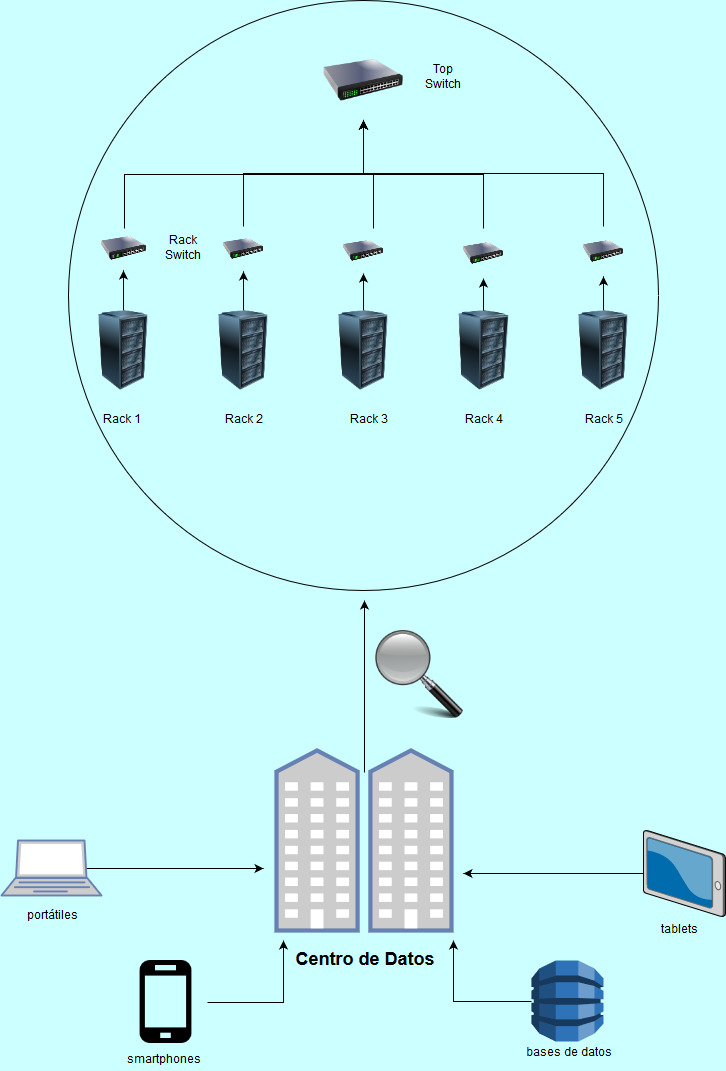
\includegraphics[scale=0.5]{C:/Users/David/Desktop/TFG/TFGLatex/imagenes/cluster_topology.jpg}
  \caption[Topología de un \textit{cluster}]{Topología de un \textit{cluster}}
  \label{cluster_topology}
\end{figure}

\clearpage


\section{Topología de un \textit{cluster Hadoop}}
Como se ha mencionado en la \autoref{sec:que_es_apache_hadoop}, \textit{Hadoop} este se compone de dos partes 
fundamentales. Cada una de esas partes se compone de subprocesos que se encargan de distintas tareas por lo que
lo primero que debemos hacer es elegir máquinas con una configuración de \textit{hardware} 
adecuada a los servicios que se va a desplegar en ella.

En \textit{clusters} destinados a producción, la mejor opción es utilizar \textit{Cloudera Manager} para
su despliegue. El asistente gráfico y todos los servicios que lleva por detrás irán instalados en una
sola máquina. \\
El resto de servicios propios de \textit{Hadoop} pueden ser instalados en una sola máquina (esto se conoce 
como modo pseudodistribuido\index{Pseudodistribuido}) o en varias máquinas (modo distribuido).
Como regla general, se necesitan mínimo dos máquinas \textit{master}, tres máquinas \textit{worker} y una
máquina \textit{gateway} para tener un \textit{cluster} plenamente funcional.
\newline

Respecto a los servicios de \textit{HDFS} y \textit{YARN} hay que tener ciertas consideraciones,
por ejemplo, la máquina designada como \textit{NameNode} necesitará mas memoria \textit{RAM} 
debido a que este guarda toda la información de los metadatos de los archivos en memoria. 
También, las máquinas que designemos como trabajadoras será recomendable que tengan buenos recursos 
de \textit{CPU} y memoria así como conexión de red de alta velocidad, de esta manera los trabajos 
que subamos al \textit{cluster} se ejecutaran de manera mas rápida.
Las máquinas \textit{worker} será muy recomendable que lleven instalados los servicios de 
\textit{NodeManager} y \textit{DataNode} conjuntamente, si bien no es obligatorio.
Para un conocimiento mas profundo acerca de los servicos de \textit{Hadoop}, ver 
\url{http://hadoop.apache.org/docs/current/}
\newline

A continuación, se muestra un esquema de un \textit{cluster Hadoop} con una configuración básica de los dos 
servicios mencionados anteriormente.

\begin{figure}[h]
  \centering
  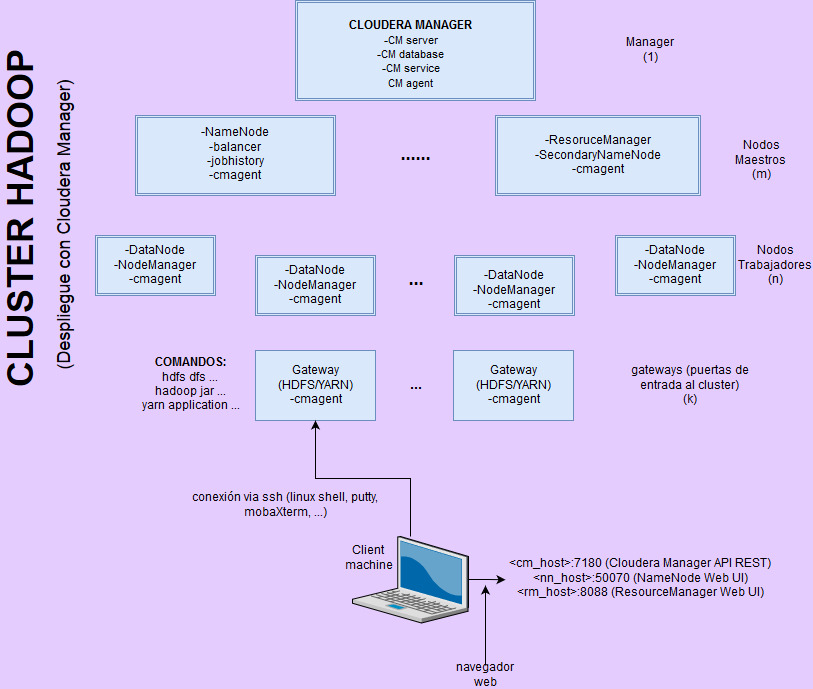
\includegraphics[scale=0.5]{C:/Users/David/Desktop/TFG/TFGLatex/imagenes/hadoop_topology.jpg}
  \caption[Servicios de un \textit{cluster Hadoop}]{Servicios de un \textit{cluster Hadoop}}
  \label{hadoop_topology}
\end{figure}

\clearpage

%%%%%%%%%%%%%%%%%%%%%%%%%%%%%%%%%%%%%%%%%%%%%%%%%%%%%%%%%%%%%%%%%%
%%%%%%%%%%%%%%%%%%%%%% CAPITULO 2 %%%%%%%%%%%%%%%%%%%%%%%%%%%%%%%%
%%%%%%%%%%%%%%%%%%%%%%%%%%%%%%%%%%%%%%%%%%%%%%%%%%%%%%%%%%%%%%%%%%


\chapter{Instalación y despliegue de un \textit{cluster}}
En esta sección vamos a preparar las máquinas para albergar un \textit{cluster} y 
posteriormente instalar el software \textit{Hadoop} en ellas.
Previamente a la instalación de \textit{Hadoop} hay que preparar las máquinas con los requisitos 
necesarios para el correcto funcionamiento.\\
La instalación se ha realizado en 7 máquinas con las siguientes características:

\begin{table}[!htbp]
  \centering
  \begin{tabular}{|r|c|c|c|c|} % tabla
    \hline
    & \textcolor{Orange}{1 \textit{Manager}} & \textcolor{OliveGreen}{2 \textit{masters}} & \textcolor{BrickRed}{3 \textit{workers}} & \textcolor{blue}{1 \textit{gateway}} \\ \hline
    Sistema Operativo & CentOS 7 & CentOS 7 & CentOS 7 & CentOS 7 \\ \hline
    \textit{CPU} & 2 vcores & 2 vcores & 4 vcores & 2 vcores \\ \hline
    Memoria & $8gb$ & $4gb$ & $8gb$ & $4gb$ \\ \hline
    Disco duro & $40gb$ & $20gb$ & $80gb$ & $20gb$ \\ \hline
    \textit{GPU} & None & None & None & None \\ \hline
    \textit{Java} & $1.8.0\_101$ & $1.8.0\_101$ & $1.8.0\_101$ & $1.8.0\_101$ \\ \hline
    \textit{Python} & $2.7$ & $2.7$ & $2.7$ & $2.7$ \\ \hline
    Versión \textit{CDH} & $5$ & $5$ & $5$ & $5$ \\ \hline
  \end{tabular}
  \caption[\textit{Hardware} de las máquinas del \textit{cluster}]{Especificaciones de las máquinas}
  \label{cluster_machines_specification}
\end{table}

Con las máquinas disponibles lo primero que debemos hacer es elegir que máquina albergará cada rol dentro 
del \textit{cluster}, esto vendrá dado por los recursos disponibles de cada nodo y el uso que pretendamos hacer.
Hay que tener en cuenta que \textit{Hadoop} es escalable por lo que nuestro \textit{cluster} podrá 
ser ampliado en número de nodos según sea la demanda de recursos que necesitemos.\\
En nuestro caso, el reparto de roles queda así:

\begin{table}[!htbp]
  \centering Roles en el \textit{cluster} %texto cabecera
  \begin{tabular}{|r|c|c|c|c|c|c|c|} % tabla
    \hline
    & Master1 & Master2 & Worker1 & Worker2 & Worker3 & Gateway & Manager \\ \hline
    \textit{namenode} & \textcolor{OliveGreen}{\checkmark}  &  &  &  &  &  & \\ \hline
    \textit{secondary namenode} &  & \textcolor{OliveGreen}{\checkmark} &  &  &  &  & \\ \hline
    \textit{datanode} &  &  & \textcolor{BrickRed}{\checkmark} & \textcolor{BrickRed}{\checkmark} & \textcolor{BrickRed}{\checkmark} & & \\ \hline
    \textit{hdfs gateway} &  &  &  &  &  & \textcolor{Blue}{\checkmark} & \\ \hline
    \textit{resource manager} &  & \textcolor{OliveGreen}{\checkmark} &  &  &  &  & \\ \hline
    \textit{node manager} &  &  & \textcolor{BrickRed}{\checkmark} & \textcolor{BrickRed}{\checkmark} & \textcolor{BrickRed}{\checkmark} &  & \\ \hline
    \textit{job history server} & \textcolor{OliveGreen}{\checkmark} &  &  &  &  &  & \\ \hline
    \textit{yarn gateway} &  &  &  &  &  & \textcolor{Blue}{\checkmark} & \\ \hline
    
	\textit{cm server} & & & & & & & \textcolor{Orange}{\checkmark} \\ \hline
	\textit{cms database} & & & & & & & \textcolor{Orange}{\checkmark} \\ \hline
	\textit{cm service} & & & & & & & \textcolor{Orange}{\checkmark} \\ \hline
	\textit{cm agent} & \textcolor{Orange}{\checkmark} & \textcolor{Orange}{\checkmark} & \textcolor{Orange}{\checkmark} & \textcolor{Orange}{\checkmark} & \textcolor{Orange}{\checkmark} & \textcolor{Orange}{\checkmark} & \textcolor{Orange}{\checkmark} \\ \hline
    
  \end{tabular}
  \caption[Asignación de roles en el \textit{cluster}]{Asignación de roles entre máquinas}
  \label{asignacion_roles_cluster}
\end{table}

% Instalación de java y demás requisitos antes de instalar el software (cloudera repo, bases de datos, selinux, ...)
Como pasos previos a la instalación de los servicios del \textit{cluster}, se deben configurar 
ciertas propiedades del Sistema Operativo\index{Sistema Operativo} tales como parar el servicio \textit{iptables},
instalación de \href{https://es.wikipedia.org/wiki/Network_Time_Protocol}{NTP} para la sincronización de relojes, 
instalar el repositorio de \textit{Cloudera}, ...
Además de todo esto, debemos instalar Java ya que \textit{Hadoop} lo requiere para poder funcionar.

\clearpage

Todo este trabajo, si bien no es complicado, excede la longitud y los objetivos de este documento, por lo que he
omitido la inclusión de esta parte a la cual se puede acceder a través del siguiente link: 
\url{https://github.com/davidRetana/custom_centOS}
\newline

% Dar nombre a las máquinas
Antes de instalar el \textit{software}, tenemos que dar nombre a cada una de las máquinas que formaran el \textit{cluster}.
Esto se hace mapeando en el archivo \path{/etc/hosts} cada ip\index{IP} de la máquina con el nombre que la queramos dar.
%De aquí en adelante los comando de \textit{UNIX}\index{UNIX} donde haya que rellenar opciones se marcaran entre < >

\begin{lstlisting}[language=bash, numbers=none]
$ sudo vi /etc/hosts
\end{lstlisting}

\begin{figure}[!htpb]
  \centering
  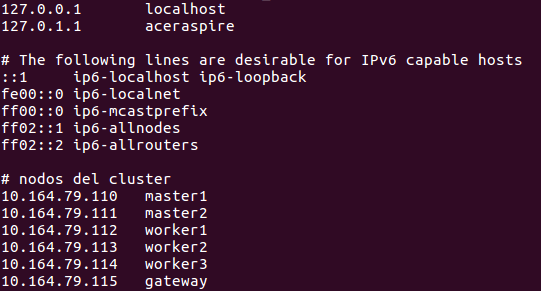
\includegraphics[width=\textwidth]{C:/Users/David/Desktop/TFG/TFGLatex/imagenes/etc_hosts.png}
  %\caption[archivo \path{/etc/hosts}]{resultado del archivo \path{/etc/hosts}}
  \label{etc_hosts}
\end{figure}

A continuación copiamos el archivo a cada máquina del \textit{cluster}:
\begin{lstlisting}[language=bash, numbers=none]
$ sudo scp /etc/hosts root@<ip_maquina_destino>:/etc/hosts
\end{lstlisting}

Para cada máquina del \textit{cluster} hacer:
\begin{lstlisting}[language=bash, numbers=none]
$ sudo hostname <nombre_de_la_maquina>
$ sudo vi /etc/sysconfig/network
\end{lstlisting}
En el archivo \path{/etc/sysconfig/network} cambiar HOSTNAME=<nombre máquina>
\newline

Para probar que los nodos se reconocen por su nombre lanzar el siguiente comando:
\begin{lstlisting}[language=bash, numbers=none]
$ ping <nombre_nodo_destino>
\end{lstlisting}
Si el nodo responde, lo hemos configurado bien.
\newline

% COMIENZO INSTALACION SOFTWARE
Para comenzar el despliegue del \textit{cluster}, instalaremos los dos servicios fundamentales para su 
correcto funcionamiento y sobre ellos se podrán añadir más servicios en un futuro. 
Sin embargo, este no es el objetivo del documento, y nos centraremos en instalar \textbf{\textit{HDFS}}, 
\textbf{\textit{YARN}} y posteriormente \textbf{\textit{Spark}}. 

\clearpage

\section{Instalación de \textit{HDFS} y \textit{YARN}}\label{sec:instalacion_hdfs_yarn}

En la máquina designada como Cloudera Manager instalamos el servicio de \textit{cloudera manager server}

\begin{lstlisting}[language=bash, numbers=none]
$ sudo yum install cloudera-manager-server
\end{lstlisting}

Este comando nos instala el servicio en la máquina en cuestión. Una vez finalizado, se nos habrá creado el
directorio \path{/usr/share/cmf} dentro del cual tenemos que lanzar un \textit{script} que nos configura la base de 
datos que usa Cloudera Manager por debajo

\begin{lstlisting}[language=bash, numbers=none]
$ sudo /usr/share/cmf/schema/scm-prepare-database.sh <base_de_datos> <nombre_db> \
  <usuario> <password>
\end{lstlisting}

A modo de ejemplo:

%\begin{listing}[style=consola, numbers=none, escapeinside={\textbackslash}]
%\$ sudo /usr/share/cmf/schema/scm-prepare-database.sh mysql cloudera root training
%\end{listing}

\begin{lstlisting}[language=bash, numbers=none]
$ sudo /usr/share/cmf/schema/scm-prepare-database.sh mysql cloudera root training
\end{lstlisting}

Si todo a funcionando correctamente, accedemos a \textit{mysql}\footnote{Sistema de gestión de base de datos relacional}\index{MySql} y vemos que se hayan creado correctamente las tablas

\begin{lstlisting}[language=bash, numbers=none]
$ mysql -uroot -ptraining

  mysql > show databases;
  mysql > exit;
\end{lstlisting}

Deberemos ver como las bases de datos \textit{amon} y \textit{rman} están creadas.\\
Finalmente arrancamos el servicio del \textit{cloudera-manager-server}

\begin{lstlisting}[language=bash, numbers=none]
$ sudo service cloudera-scm-server start
\end{lstlisting}

Este proceso tarda en terminar de ejecutarse pero una vez finalizado nos abrimos un navegador desde nuestro
portátil y escribimos en el campo de la url: \path{<ip_nodo_cloudera_manager>:7180}\\
A partir de ahora, será el asistente gráfico el que nos guíe a través del proceso de instalación del
\textit{cluster} en el resto de las máquinas. Para hacer el login inicial escribimos usuario:admin y 
password:admin, de esta manera ya estamos dentro del asistente gráfico.

\begin{figure}[!htpb]
  \centering
  \includegraphics[scale=0.5]{C:/Users/David/Desktop/TFG/TFGLatex/imagenes/capturas_cm/Captura1.JPG}
  %\caption[archivo \path{/etc/hosts}]{resultado del archivo \path{/etc/hosts}}
\end{figure}

Como se comento previamente, Cloudera Manager es un software gratuito pero en su versión Cloudera Express,
sin embargo, tiene una versión de pago llamada Cloudera Enterprise con funciones avanzadas para la gestión del
\textit{cluster} además de soporte. Esta opción esta disponible durante un mes a modo de prueba gratuita.
\newline

A lo largo de toda la instalación nos pedirá diversas opciones de configuración como por ejemplo el uso de
remesas de Cloudera, que son sencillamente abstracciones a nivel de repositorios de paquetes para que
podamos tener diferentes versiones de un mismo software sin que entren en conflicto y poder elegir que
versión usar en cada momento.
\newline

Como Cloudera Manager necesita acceder a los nodos para desplegar paquetes de software e instalar agentes, necesita
acceder por \textit{SSH} a las máquinas por lo que nos pedirá la contraseña de los nodos del \textit{cluster}.
En este caso dicha contraseña deberá ser igual en todos los nodos.

\clearpage

\begin{figure}[!htpb]
  \centering
  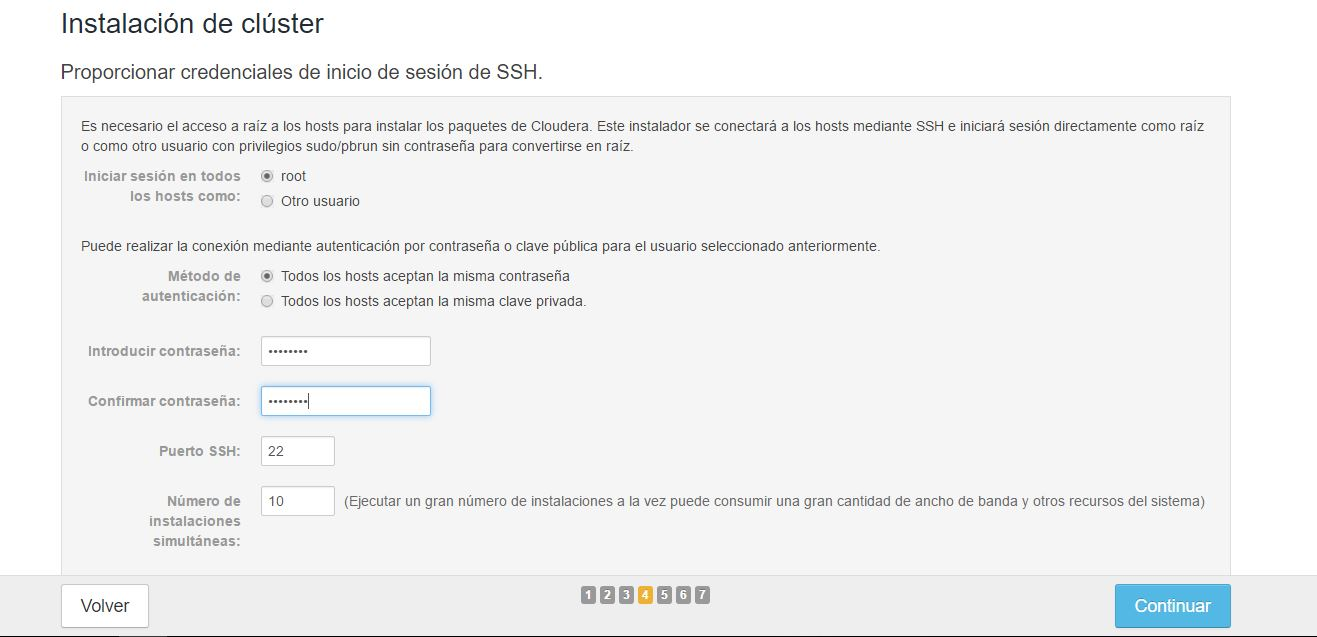
\includegraphics[width=\textwidth]{C:/Users/David/Desktop/TFG/TFGLatex/imagenes/capturas_cm/Captura8.JPG}
  %\caption[archivo \path{/etc/hosts}]{resultado del archivo \path{/etc/hosts}}
\end{figure}

A continuación se comenzará a descargar los paquetes de código y distribuirlos por las máquinas

\begin{figure}[!htpb]
  \centering
  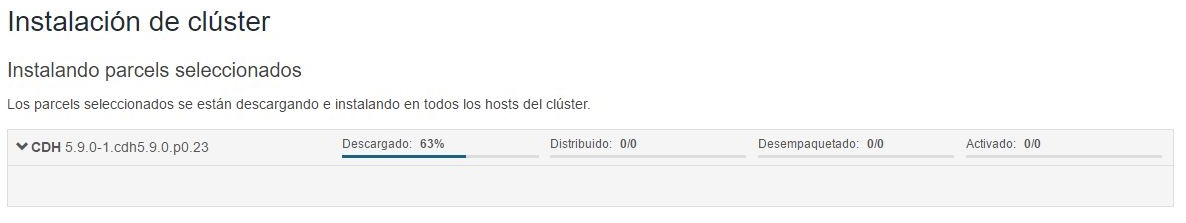
\includegraphics[width=\textwidth]{C:/Users/David/Desktop/TFG/TFGLatex/imagenes/capturas_cm/Captura11.JPG}
  %\caption[archivo \path{/etc/hosts}]{resultado del archivo \path{/etc/hosts}}
\end{figure}

Si todo funciona correctamente deberemos ver una pantalla como la siguiente:

\begin{figure}[!htpb]
  \centering
  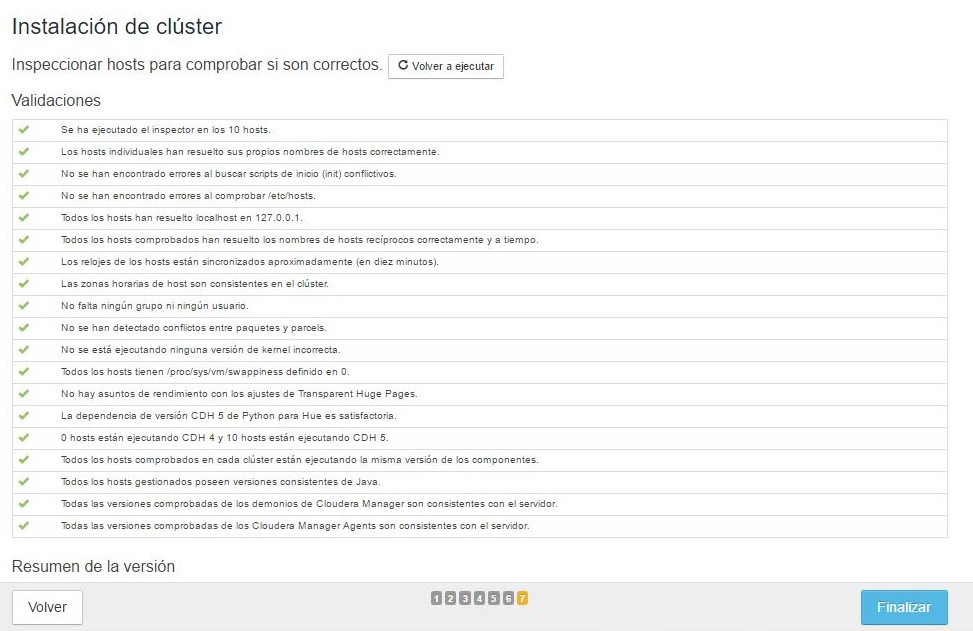
\includegraphics[width=\textwidth]{C:/Users/David/Desktop/TFG/TFGLatex/imagenes/capturas_cm/Captura16.JPG}
  %\caption[archivo \path{/etc/hosts}]{resultado del archivo \path{/etc/hosts}}
\end{figure}

Esta pantalla nos indica que todo ha salido correctamente. Comprueba entre otras cosas que los requisitos
mencionados al inicio del capítulo se cumplen y el despliegue del software ha sido satisfactorio.
\newline

Posteriormente, en la elección de los servicios a desplegar seleccionamos \textit{HDFS} y \textit{YARN} e
indicamos los nodos donde queremos que se instalen acorde a la \autoref{asignacion_roles_cluster}.\\
A continuación rellenamos las propiedades de los directorios donde los servicios de \textit{HDFS} y \textit{YARN}
dejarán los datos y habremos finalizado la instalación del \textit{cluster}.

\begin{figure}[!htpb]
  \centering
  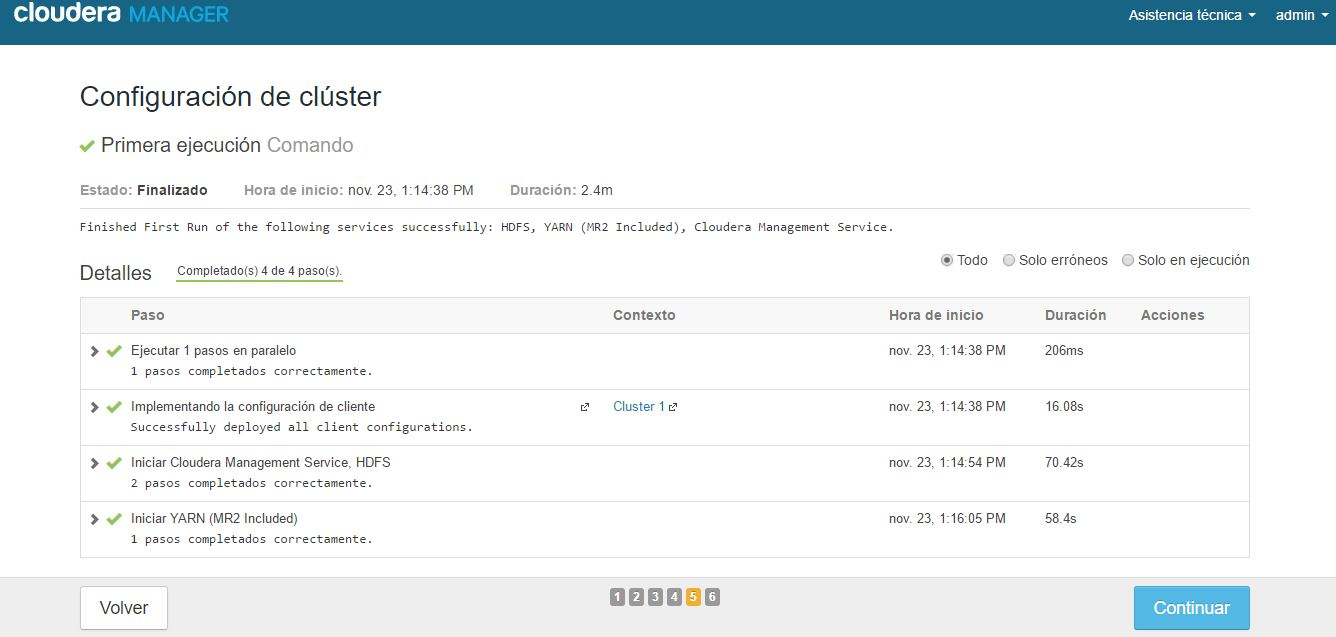
\includegraphics[width=\textwidth]{C:/Users/David/Desktop/TFG/TFGLatex/imagenes/capturas_cm/Captura23.JPG}
  %\caption[archivo \path{/etc/hosts}]{resultado del archivo \path{/etc/hosts}}
\end{figure}

Si todo fue satisfactoriamente, deberemos ser redirigidos a la página principal de administración de
Cloudera Manager. Esta página será el punto de partida para cualquier configuración que queramos hacer
en el \textit{cluster}, así como añadir nuevos nodos, desplegar nuevos servicios, habilitar la alta
disponibilidad en el \textit{cluster} (HA\index{HA} por sus siglas en inglés 
\textit{High Availability}\footnote{Consiste en habilitar un segundo \textit{namenode} en el \textit{cluster} 
para evitar que un fallo en el nodo \textit{namenode} deje fuera de servicio al \textit{cluster} entero.}), ...\\
Además permite obtener métricas del uso de \textit{CPU}, I/O de red y de disco, etc.

\begin{figure}[!htpb]
  \centering
  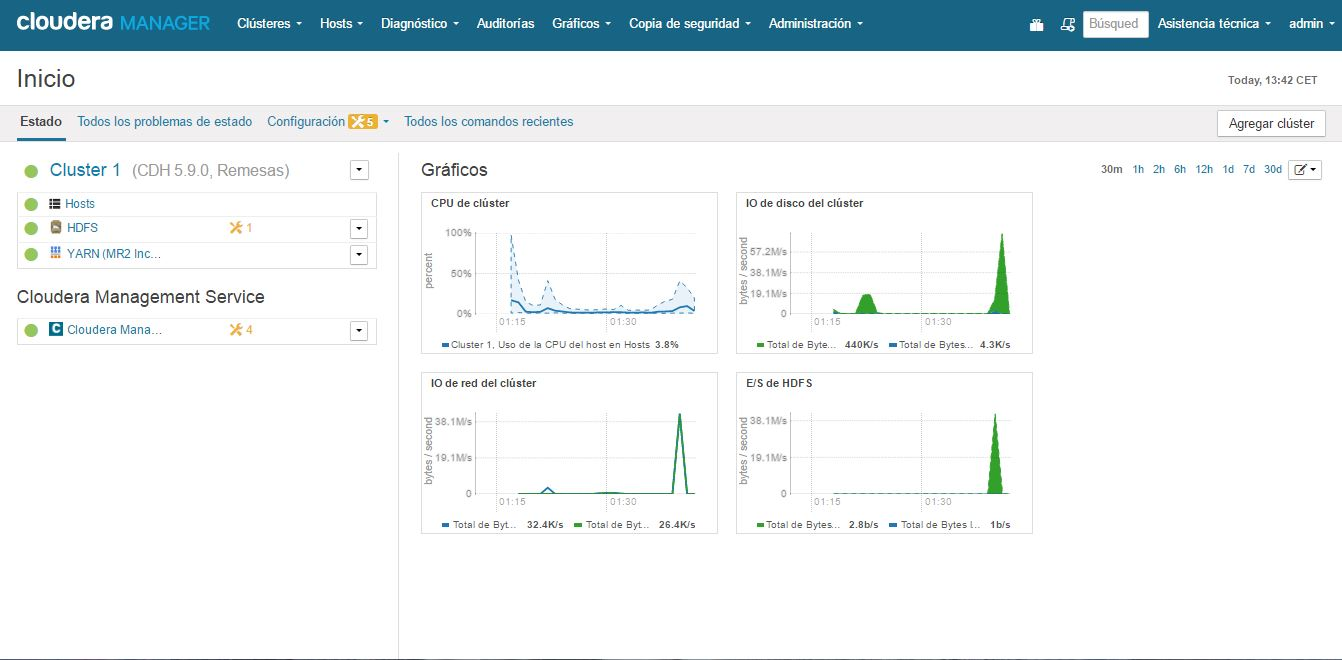
\includegraphics[width=\textwidth]{C:/Users/David/Desktop/TFG/TFGLatex/imagenes/capturas_cm/Captura26.JPG}
  \caption[Instantánea Cloudera Manager]{Instantánea de la pagina principal de Cloudera Manager}
\end{figure}

\subsection{Test del \textit{cluster} desplegado}\label{test_cluster_desplegado}
Para comprobar el correcto funcionamiento del \textit{cluster} instalado con Cloudera Manager, vamos a subir
un archivo a \textit{HDFS}, veremos como se distribuye entre los nodos (en porciones de $128$ \textit{MB} por defecto) 
y luego ejecutaremos un trabajo \textit{MapReduce} que es el motor por defecto que utiliza \textit{YARN v2}.

\clearpage

Logeados en nuestra máquina \textit{gateway}, lo primero que debemos hacer es crearnos un directorio de trabajo
en \textit{HDFS} para nuestro usuario y darle permisos. Ademas vamos a crear un directorio temporal donde
todos los usuarios puedan escribir.

\begin{lstlisting}[language=bash, numbers=none]
$ # creacion de la home del usuario
$ sudo -u hdfs hdfs dfs -mkdir -p /user/<nombre_usuario>
$ sudo -u hdfs hdfs dfs -chown -R <nombre_usuario> /user/<nombre_usuario>
$ # creacion del directorio temporal
$ sudo -u hdfs hdfs dfs -mkdir -p /tmp
$ sudo -u hdfs hdfs dfs -chmod -R 1777 /tmp
\end{lstlisting}

Hecho esto, lanzamos el comando para subir un archivo que esta en local a \textit{HDFS} y luego comprobamos
que realmente se ha subido:

\begin{lstlisting}[language=bash, numbers=none]
$ hdfs dfs -put <path_archivo_local> <path_en_hdfs>
$ hdfs dfs -ls
\end{lstlisting}

Si todo ha funcionado correctamente, abrimos un navegador y escribimos \path{<ip_namenode>:50070}

\begin{figure}[!htpb]
  \centering
  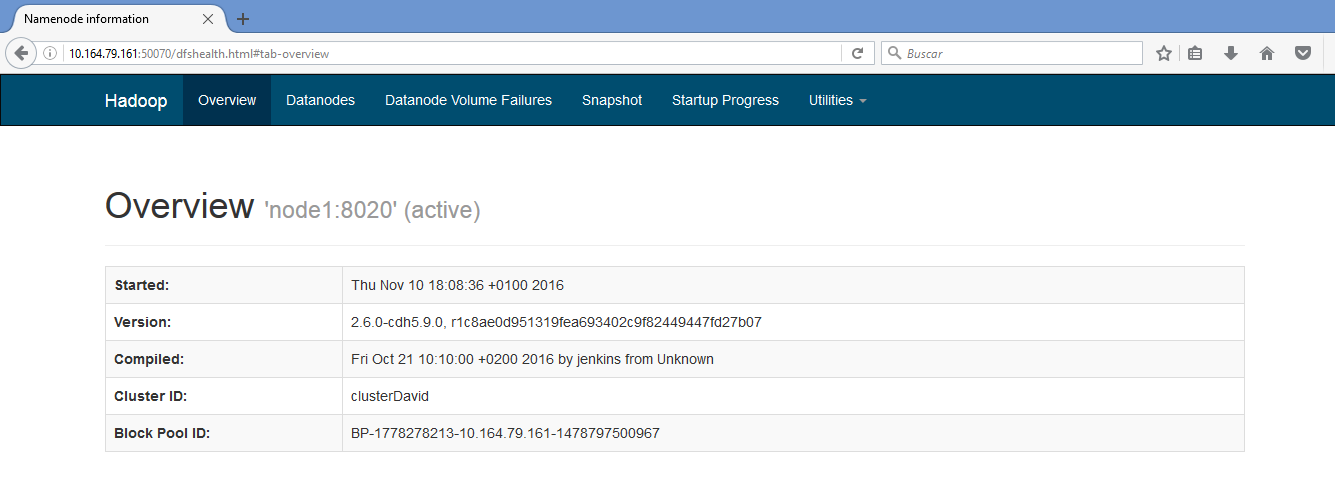
\includegraphics[width=\textwidth]{C:/Users/David/Desktop/TFG/TFGLatex/imagenes/capturas_creacion_cluster/1.png}
  \caption[\textit{Overview web namenode}]{\textit{Overview} del servicio web del \textit{namenode}}
\end{figure}

Si nos vamos a la pestaña de \textit{Datanodes} veremos los nodos trabajadores que tenemos activos y su 
capacidad de almacenamiento entre otras cosas.

\begin{figure}[!htpb]
  \centering
  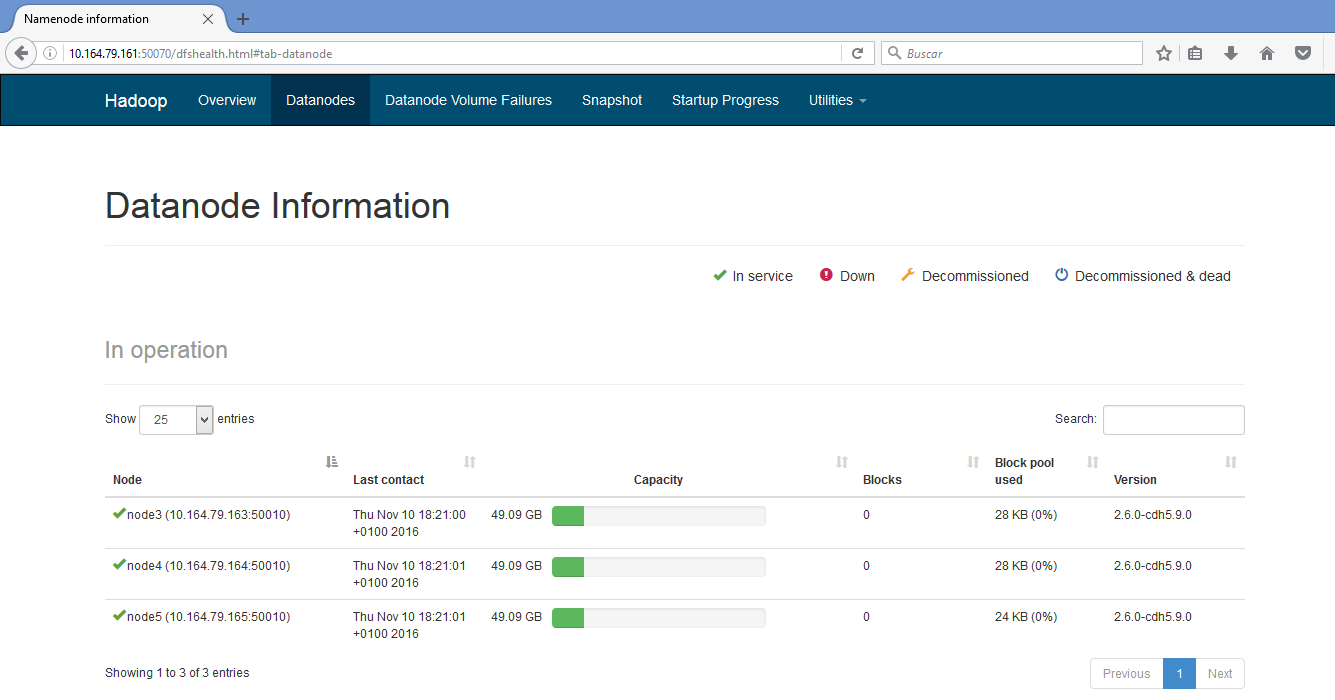
\includegraphics[width=\textwidth]{C:/Users/David/Desktop/TFG/TFGLatex/imagenes/capturas_creacion_cluster/5.png}
  \caption[Información web \textit{Datanode}]{Información de los \textit{datanodes}}
\end{figure}

\clearpage

Para testear \textit{YARN}, vamos a lanzar un trabajo \textit{MapReduce} en dos fases, una primera donde
solo se ejecute la fase \textit{map} y luego otra donde solo se ejecute la fase \textit{reduce}.

\begin{lstlisting}[language=bash, numbers=none]
$ hadoop jar /usr/lib/hadoop-mapreduce/hadoop-mapreduce-examples-2.6.0-cdh5.9.0.jar \
   teragen 10000 output_prueba_teragen
\end{lstlisting}

Veremos una salida parecida a esta:

\begin{figure}[!htpb]
  \centering
  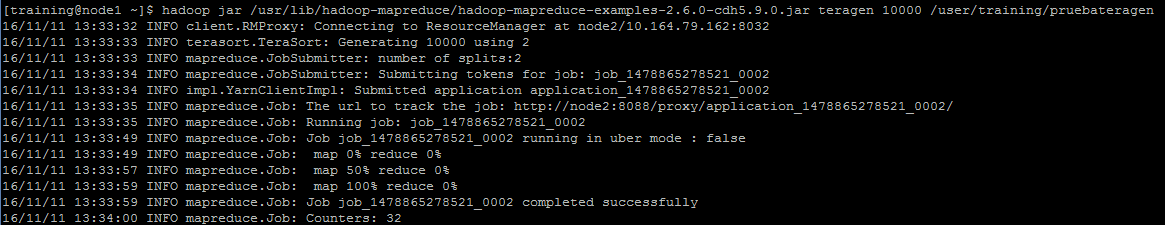
\includegraphics[width=\textwidth]{C:/Users/David/Desktop/TFG/TFGLatex/imagenes/capturas_creacion_cluster/12.png}
  %\caption[archivo \path{/etc/hosts}]{resultado del archivo \path{/etc/hosts}}
\end{figure}

Ahora ejecutaremos la fase reduce donde recibirá como entrada la salida del trabajo anterior

\begin{lstlisting}[language=bash, numbers=none]
$ hadoop jar /usr/lib/hadoop-mapreduce/hadoop-mapreduce-examples-2.6.0-cdh5.9.0.jar \
   terasort output_prueba_teragen output_prueba_terasort
\end{lstlisting}

Donde nuevamente veremos una salida parecida a esta:

\begin{figure}[!htpb]
  \centering
  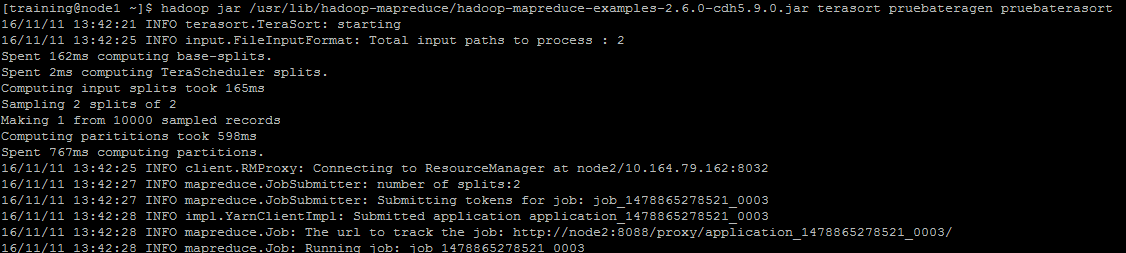
\includegraphics[width=\textwidth]{C:/Users/David/Desktop/TFG/TFGLatex/imagenes/capturas_creacion_cluster/15.png}
  %\caption[archivo \path{/etc/hosts}]{resultado del archivo \path{/etc/hosts}}
\end{figure}

Si nos vamos a un navegador y escribimos \path{<ip_resourcemanager>:8088}, veremos de una manera gráfica
los trabajos que se están ejecutando en nuestro \textit{cluster}, el historial de trabajos subidos, la
memoria utilizada, los contenedores asignados, ...\\
Llegados a este punto, ya tendremos un \textit{cluster} totalmente operativo con los servicios de
\textit{HDFS} Y \textit{YARN} instalados correctamente.

\begin{figure}[!htpb]
  \centering
  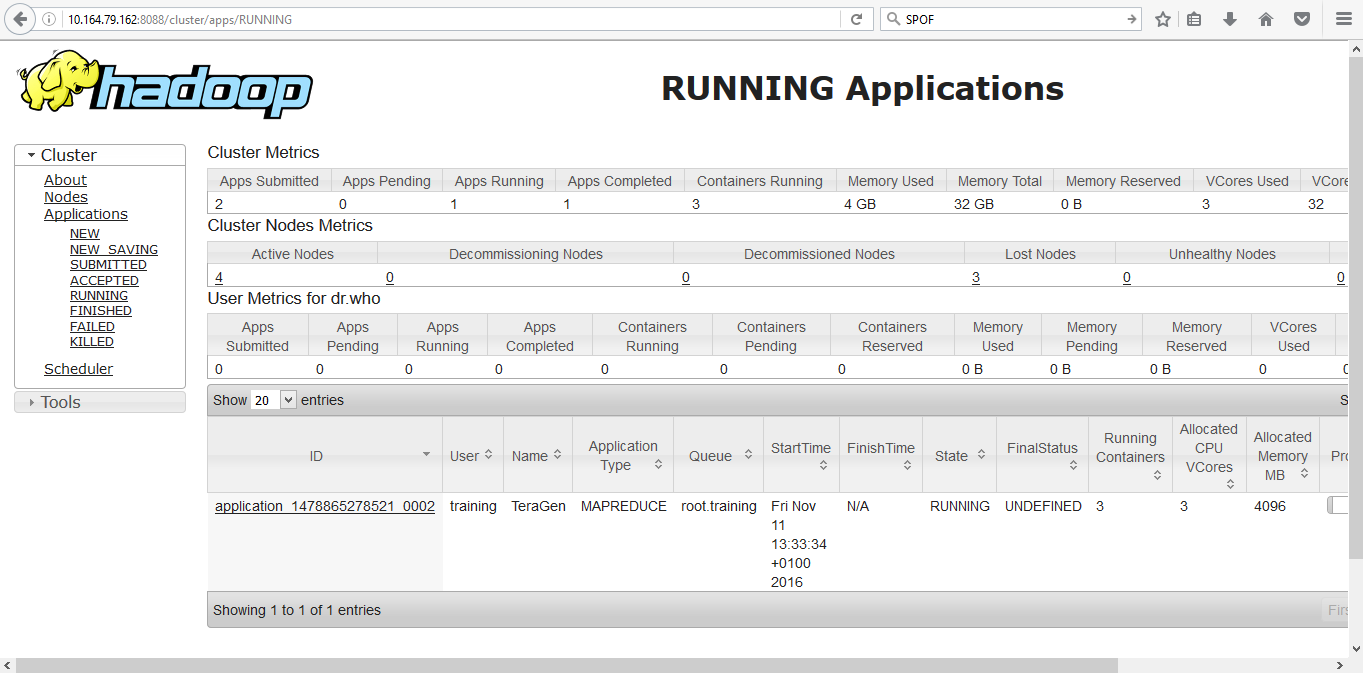
\includegraphics[width=\textwidth]{C:/Users/David/Desktop/TFG/TFGLatex/imagenes/capturas_creacion_cluster/11.png}
  \caption[Web del servicio \textit{Resource Manager}]{Web del servicio \textit{resource manager}}
\end{figure}

\clearpage

\section{Instalación de \textit{Apache Spark}}\label{sec:instalacion_spark}
             
%\begin{wrapfigure}[lineheight]{position}{width}
\begin{wrapfigure}[]{l}{0.5\textwidth}
  \centering
  \includegraphics[width=0.5\textwidth]{C:/Users/David/Desktop/TFG/TFGLatex/imagenes/capturas_spark/Captura1.JPG}
\end{wrapfigure}

Para la instalación de \textit{Apache Spark}, desde la página principal de administración de Cloudera Manager
seleccionamos la pestaña 'Agregar un servicio' en el desplegable de \textit{cluster}.
En esta pestaña están disponible todos los servicios soportados por Cloudera y que por lo tanto son compatibles
con nuestro \textit{cluster}.\\
Nota: Ya se encuentra disponible la version $2.0$ de \textit{Spark}, pero su
instalación es algo diferente ya que debe hacerse desde las \textit{parcels} de Cloudera. Esto es así porque
las versiones $2.x.x$ son incompatibles con las versiones $1.x.x$
\newline

La opción de \textit{Spark} que cogeremos será aquella que utilice \textit{YARN} como gestor de recursos del
\textit{cluster}.
Notese que la opción \textit{Spark} (\textit{Standalone}\footnote{\textit{Standalone} es un modo de despliegue
autónomo, no requiere de ningún gestor de recursos del \textit{cluster}.}
\index{Standalone}) también está disponible.

\begin{figure}[!htpb]
  \centering
  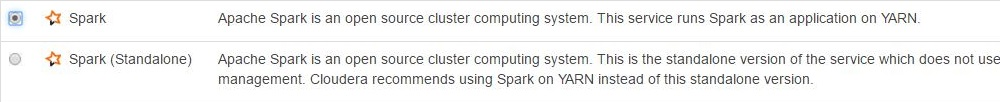
\includegraphics[width=\textwidth]{C:/Users/David/Desktop/TFG/TFGLatex/imagenes/capturas_spark/Captura2.JPG}
\end{figure}

Una vez hecho esto, elegimos la máquina que hemos etiquetado como \textit{gateway} para desplegar el servicio
de \textit{Spark} ya que será desde esta máquina donde subiremos nuestros trabajos 
\textit{spark-submit}\index{Spark-submit} o \textit{pyspark}\index{Pyspark} al \textit{cluster}.
Después de todo este proceso de instalación, nuestra pagina principal de Cloudera Manager debería lucir los 
3 servicios que hemos instalado.

\begin{figure}[!htpb]
  \centering
  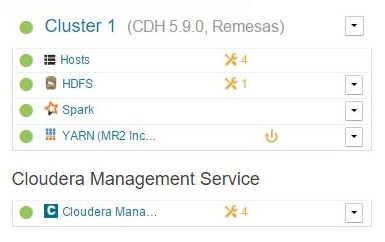
\includegraphics[width=0.6\textwidth]{C:/Users/David/Desktop/TFG/TFGLatex/imagenes/capturas_spark/Captura5.JPG}
\end{figure}

Lo ultimo que nos queda por hacer es reiniciar el servicio de \textit{YARN} para que hagan efecto
los cambios que hemos realizado en el \textit{cluster}.

\begin{figure}[!htpb]
  \centering
  
\includegraphics[width=0.6\textwidth]{C:/Users/David/Desktop/TFG/TFGLatex/imagenes/capturas_spark/Captura5_paint.JPG}
\end{figure}

Seguimos el asistente de reinicio y habremos terminado la instalación de \textit{Spark}.
\newline

Para comprobar su correcto funcionamiento iniciamos un intérprete \textit{pyspark} desde la máquina \textit{gateway}
\begin{lstlisting}[language=bash, numbers=none]
$ pyspark --master local[*]
\end{lstlisting}

\clearpage

\begin{figure}[!htpb]
  \centering
  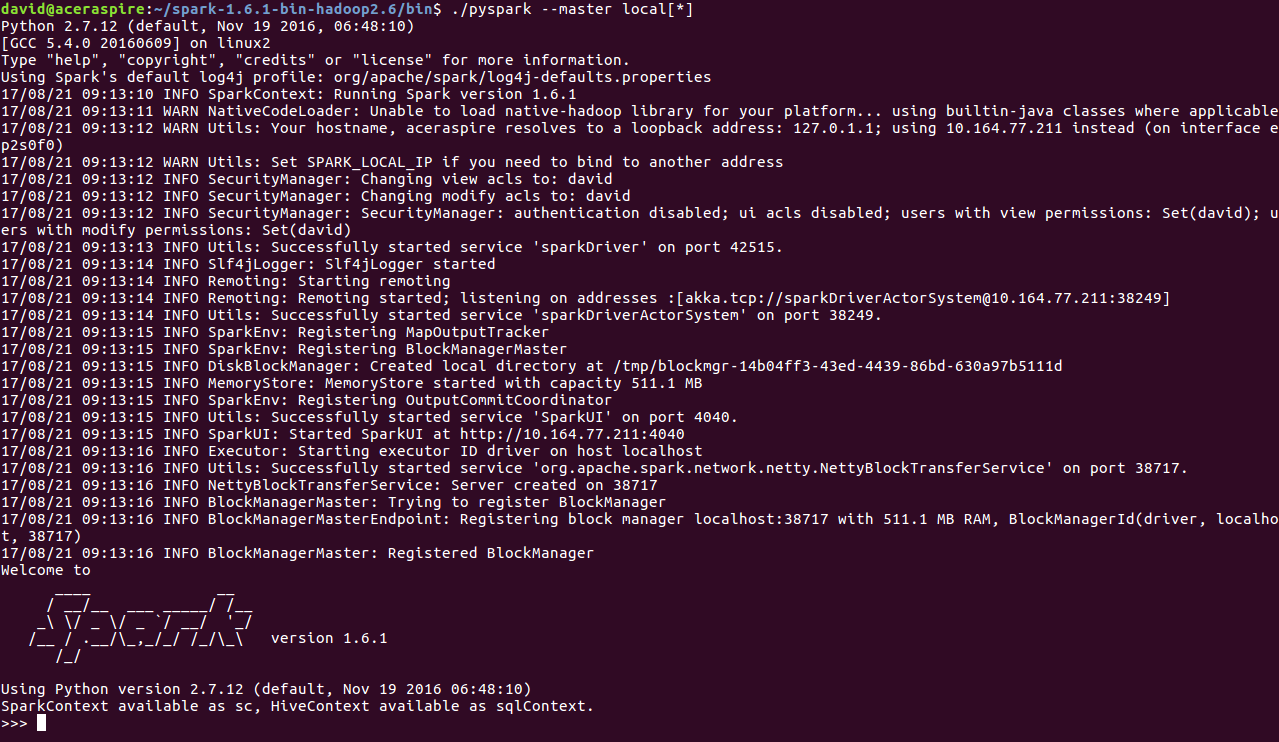
\includegraphics[width=\textwidth]{C:/Users/David/Desktop/TFG/TFGLatex/imagenes/pyspark_shell.png}
  \caption[\textit{Pyspark shell}]{\textit{Pyspark shell}}
  \label{pyspark_shell}
\end{figure}

En esta terminal tendremos creadas por defecto las variables \textit{sc} (\textit{Spark Context}\index{Spark Context})
y \textit{sqlContext}\index{SqlContext}. La primera es el punto de partida para una aplicación \textit{Spark}, mientras
que la segunda habilita características de SQL para el tratamiento de datos.\\
Si queremos comprobar que todo funciona correctamente podemos ejecutar las siguientes ordenes de \textit{pyspark}:

\begin{lstlisting}[language=bash, numbers=none]
 >>> rdd = sc.parallelize(range(100))
 >>> rdd.count()
\end{lstlisting}

Con estas ordenes lo que estamos diciendo es que se paralelice la lista de enteros que va desde el 0 hasta el 99,
distribuyéndola entre los nodos, y luego desencadenando una acción que es el contar el número de elementos.
Si la orden se completa, hemos instalado correctamente \textit{Spark} en nuestro \textit{cluster}.

\section*{Conclusión del despliegue}

Esto concluye el despliegue de un \textit{cluster} realizado con Cloudera Manager, donde hemos instalado los
servicios básicos de \textit{Hadoop} y además el motor de procesamiento \textit{Spark}.\\
En el siguiente capítulo se comentará las diferencias entre los distintos enfoques de procesamiento y se
explica en que consisten los \textit{frameworks} de \textit{MapReduce} y \textit{Spark}.
En la \autoref{part:analisis_datos} (\nameref{part:analisis_datos}) se utiliza el \textit{cluster} construido 
en esta sección para entrenar los modelos de \textit{machine learning} y reducir sus tiempos de ejecución.

\clearpage


%%%%%%%%%%%%%%%%%%%%%%%%%%%%%%%%%%%%%%%%%%%%%%%%%%%%%%%%%%%%%%%%%%
%%%%%%%%%%%%%%%%%%%%%% CAPITULO 3 %%%%%%%%%%%%%%%%%%%%%%%%%%%%%%%%
%%%%%%%%%%%%%%%%%%%%%%%%%%%%%%%%%%%%%%%%%%%%%%%%%%%%%%%%%%%%%%%%%%


\chapter{Computación paralela}
La computación paralela consiste en dividir el flujo de procesamiento en instrucciones que se ejecutan 
simultáneamente y de manera asíncrona con el fin de reducir los tiempos de ejecución de un programa.
Es especialmente importante hoy en día debido a la gran cantidad de datos que tratan las aplicaciones 
desarrolladas en el área del \textit{Big data}.\\
Este enfoque de programación obliga a rediseñar los algoritmos de procesamiento, en el libro \cite{DBLP:books/cu/C2017}
se encuentra una buena introducción al diseño de algoritmos paralelos.

\section[Enfoques procesamiento]{Distintos enfoques de procesamiento}\label{sec:distintos_enfoques_procesamiento}
A nivel de programación o código hay 3 enfoques de procesamiento de los datos:

\begin{itemize}
  \item Secuencial
  \item Concurrente
  \item Paralelo
\end{itemize}

A nivel de procesador también existe el concepto de paralelismo ya que las nuevas arquitecturas de \textit{microchips}
incorporan varios núcleos físicos, además cada núcleo puede manejar varios procesos a la vez 
(lo que se conoce como concurrente). Dentro de cada hilo de ejecución, las instrucciones son procesadas una a una en 
el orden en que aparecen (procesamiento secuencial).
\newline

Podemos programar de manera secuencial con \textit{Python}, de manera concurrente usando \textit{Python} y 
librerías como \textit{numpy} o \textit{multiprocessing}, o podemos programar de manera totalmente paralela
usando \textit{Python} y \textit{Apache Spark} o \textit{MapReduce} (en este último, a través de \textit{mrjob}).\\
Al ejecutar un programa básico \textit{Python}, este se ejecuta como un solo proceso. Si nuestro ordenador tiene 
por ejemplo 2 núcleos físicos (y 4 virtuales) esto quiere decir que al ejecutarse nuestro código 
este consumirá un solo núcleo virtual (\textit{virtual core} o vcore\index{Vcore}),
es decir, consumirá el $25\%$ de la capacidad de procesamiento.\\
Si queremos aprovechar el $100\% $ de la \textit{CPU} deberemos reescribir nuestro código haciendo uso de librerías 
tales como \href{https://docs.python.org/2/library/multiprocessing.html}{\textit{multiprocessing}}, 
para que el programa soporte la concurrencia y así acelerar los tiempos.
Esto por regla general no es sencillo y solo es paralelizable hasta el máximo de vcores de la \textit{CPU}. 
Algunas librerías como \href{http://www.numpy.org/}{\textit{numpy}} o 
\href{https://www.scipy.org/}{\textit{scipy}} están optimizadas para aprovechar el máximo 
de la \textit{CPU} de nuestro ordenador de manera totalmente transparente al programador.
\newline

En un sistema \textit{UNIX}, la mejor manera de comprobar la cantidad de recursos que están siendo utilizados 
por el sistema es desde una terminal ($CTRL + ALT + T$ si estamos en Ubuntu) y ejecutar el siguiente comando:

\begin{lstlisting}[language=bash, numbers=none]
$ top
\end{lstlisting}\index{Top}

Este comando muestra el consumo de recursos de cada proceso que esta corriendo en nuestra máquina.
Para monitorizar el consumo de recursos cuando se lance un proceso hay que tener en cuenta que los trabajos en 
un \textit{cluster} se distribuyen a través de los nodos, por lo que el comando \textit{top} mostrado anteriormente 
solo nos da información de la máquina donde se ha lanzado.

\clearpage

\section[Frameworks]{Frameworks de procesamiento paralelo}\label{sec:frameworks_procesamiento_paralelo}
En este trabajo nos centraremos especialmente en dos \textit{frameworks}
\footnote{\url{https://es.wikipedia.org/wiki/Framework}.}: \textit{MapReduce} y \textit{Spark}. \\
Ambos son motores de procesamiento distribuido aunque con un diseño muy diferente, que dependiendo 
de la naturaleza del problema a resolver será más conveniente utilizar uno u otro.

% MapReduce
\begin{description}
  \item[\textit{MapReduce}\index{Apache!MapReduce}:] es un \textit{framework} de procesamiento inspirado 
  en dos de las principales funciones de la programación funcional: \textit{map} y \textit{reduce}.
  \begin{itemize}
    \item \textit{map}: fase donde se produce el procesamiento en paralelo de los datos. 
          Recibe como entrada tuplas (clave, valor) $(k_x, v_x)$ y genera como salida 
          una lista de tuplas de (clave, valor) también: $[(k_1, v_1), \ldots, (k_n, v_n)]$
    \item \textit{shuffle and sort}: fase donde se produce la mezcla de las claves 
          (las claves iguales van a parar a un mismo reduce) y el ordenamiento de las mismas.
    \item \textit{reduce}: fase donde se procesa el conjunto de valores para una misma clave.
  \end{itemize}
  Adicionalmente, se pueden incorporar más fases para optimizar los trabajos \textit{MapReduce} como por
  ejemplo la utilización de \textit{combiners}\index{Combiner}\footnote{fase reduce ejecutada localmente
  en un nodo para reducir el coste del movimiento de datos a través de la red.}.\\
  \textit{MapReduce} esta incluido en \textit{YARN v2} como motor por defecto. Además, cuenta con implementaciones en 
  diversos lenguajes de programación como \textit{Java}, \textit{Scala} o \textit{Python}.\\
  Los algoritmos implementados en este trabajo se realizarán utilizando la librería \textit{mrjob} 
  de \textit{Python}, accesible a través de \url{https://pythonhosted.org/mrjob/}
\end{description}

\begin{figure}[!htpb]
  \centering
  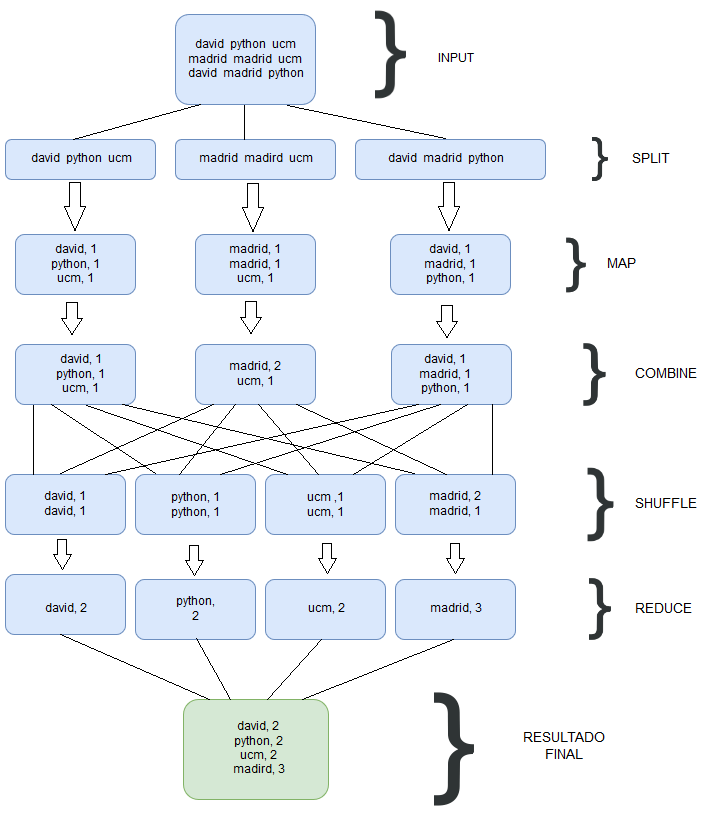
\includegraphics[scale=0.6]{C:/Users/David/Desktop/TFG/TFGLatex/imagenes/mapReduce_wordcount.png}
  \caption[Conteo de palabras en \textit{MapReduce}]{Funcionamiento interno de un \textit{word count} en \textit{MapReduce}}
  \label{mapReduce_wordcount}
\end{figure}

\clearpage

% Apache Spark
\begin{description}
  \item[\textit{Apache Spark}\index{Apache!Spark}:] es un \textit{framework} de procesamiento 
  distribuido para grandes cantidades de datos. Su diseño se basa en funciones del paradigma de programación 
  funcional, realizando los cálculos en memoria, lo que le da mayor rapidez que los motores basados en disco 
  como \textit{MapReduce}.\\
  \textit{Spark} pretende sustituir a \textit{MapReduce} como motor de procesamiento debido a su 
  mayor rendimiento, sobre todo en algoritmos iterativos, lo que acelera mucho el entrenamiento 
  de algoritmos de \textit{machine learning}.
  \textit{Spark} consta de varias librerías como \textit{ML} o \textit{MLlib} para \textit{machine learning} y 
  \textit{GraphX} para el trabajo con grafos.
  La abstracción de procesamiento en \textit{Spark} es el \textbf{RDD} (\textit{Resilient Distributed Dataset}), 
  siendo altamente escalable y tolerante a fallos (mediante puntos de control o \textit{checkpoints}).
  Además, \textit{Spark} soporta \textit{YARN} como gestor de recursos del \textit{cluster}.
  \textit{Apache Spark} es un proyecto de la \textit{Apache Software Foundation} de código abierto, descargable a 
  través de \url{https://spark.apache.org/}
\end{description}


\begin{figure}[!htpb]
  \centering
  
\includegraphics[scale=0.5]{C:/Users/David/Desktop/TFG/TFGLatex/imagenes/apache_spark.png}
  \caption[Logo \textit{Apache Spark}]{Logo de \textit{Apache Spark}}
  \label{spark-devs1}
\end{figure}

% Instalación de MRJOB
La instalación de \textit{Spark} en el \textit{cluster} se detalla en la \autoref{sec:instalacion_spark},
mientras que para la instalación de \textit{mrjob} en la máquina que hemos designado como \textit{gateway},
solo tendremos que lanzar un sencillo comando.\\

\begin{lstlisting}[language=bash, numbers=none]
$ sudo pip install mrjob
\end{lstlisting}

\textit{Pip}\footnote{\textit{Python Package Index}, \url{https://pypi.python.org/pypi/pip}.}, 
el gestor de paquetes de \textit{Python}, se encargará de descargar todas las dependencias
 necesarias para su correcta instalación.

\begin{figure}[!htpb]
  \centering
  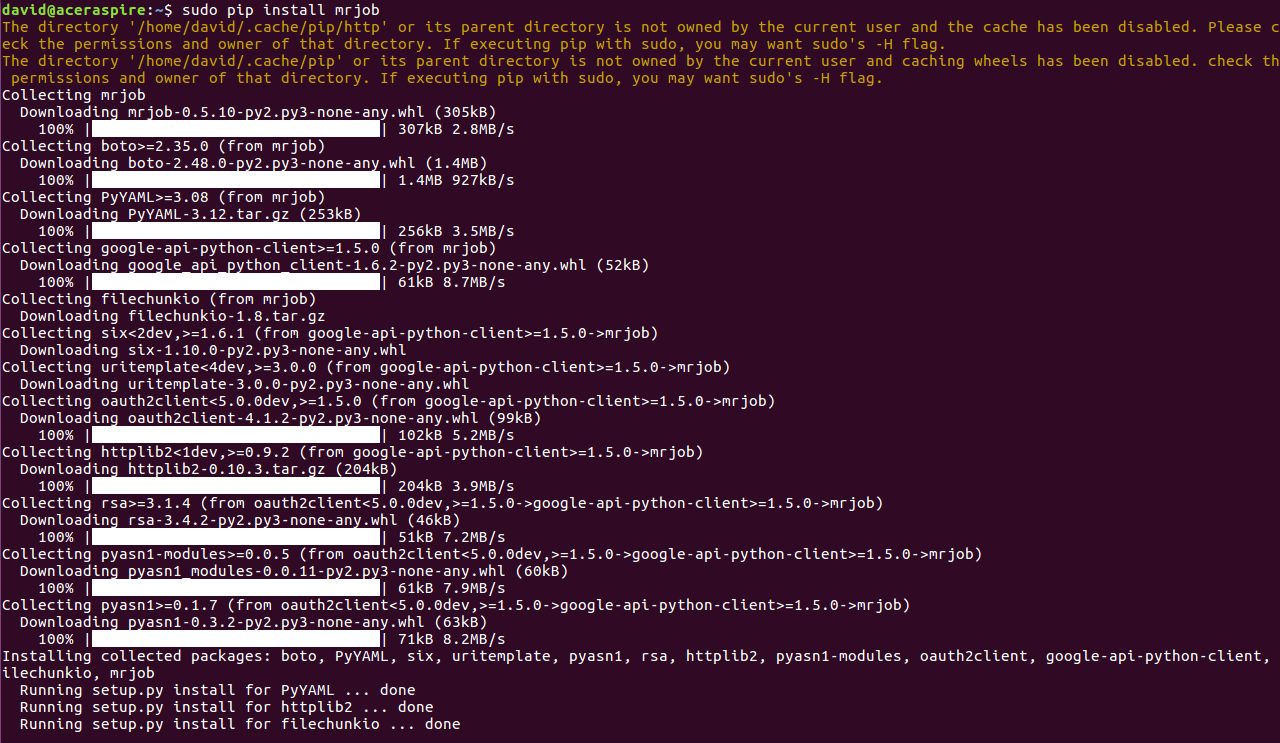
\includegraphics[width=\textwidth]{C:/Users/David/Desktop/TFG/TFGLatex/imagenes/sudo_pip_install_mrjob.png}
  \caption[Instalación de \textit{mrjob}]{Instalación de \textit{mrjob}}
  \label{sudo_pip_install_mrjob}
\end{figure}

\clearpage


%%%%%%%%%%%%%%%%%%%%%%%%%%%%%%%%%%%%%%%%%%%%%%%%%%%%%%%%%%%%%%%%%%
%%%%%%%%%%%%%%%%%%%%%%%%% PART 2 %%%%%%%%%%%%%%%%%%%%%%%%%%%%%%%%%
%%%%%%%%%%%%%%%%%%%%% CAPITULOS 4 y 5 %%%%%%%%%%%%%%%%%%%%%%%%%%%%
%%%%%%%%%%%%%%%%%%%%%%%%%%%%%%%%%%%%%%%%%%%%%%%%%%%%%%%%%%%%%%%%%%

\part{Análisis de datos}\label{part:analisis_datos}
\chapter{Machine Learning}
Los datos son una fuente de valor por lo que analizarlos y tomar decisiones en función a estos se ha
convertido en algo esencial. Cada vez son mas las compañías autodenominadas 
\textit{data-driven company}\index{Data-driven company}, es decir, empresas que toman decisiones de 
futuro e inversión en función al análisis que hacen de sus datos.\\
El \textit{machine learning} es el gran aliado de los datos ya que permite construir modelos sobre estos,
que posteriormente se usarán para tomar dichas decisiones de futuro de la compañía. A modo de ejemplo, estas
decisiones pueden ser: ¿Dónde construir un nuevo centro de datos?, ¿Cómo me anticipo a la posible baja de un
cliente de mis servicios móviles?, ¿Cómo minimizo el coste de mantenimiento de las infraestructuras?...\\
Por estas y más razones, el \textit{machine learning} y las grandes cantidades de datos manejadas en el 
\textit{Big Data} están estrechamente relacionadas.

\section{¿Qué es el machine learning?}
\textit{Machine Learning}\index{Machine Learning} (ML) es una rama de la inteligencia artificial (IA) 
que se centra en desarrollar métodos para hacer posible que los sistemas aprendan sin ser programados 
explícitamente para ello.
El denominado aprendizaje automático se basa en los datos de entrada o datos de entrenamiento, que
son utilizados para ajustar los modelos tanto predictivos, como clasificatorios, o de clusterización.

Podemos clasificar los modelos de \textit{machine learning} en dos clases:
\begin{itemize}
  \item \textbf{Aprendizaje supervisado}\index{Aprendizaje!supervisado}: los datos de entrada del 
  algoritmo van etiquetados con la salida esperada, es decir, cada dato de entrada lleva consigo 
  la clase a la que pertenece. De esta manera se pretende que el algoritmo sea capaz de identificar 
  patrones entre los datos de una misma clase para que cuando vea un dato sin etiquetar, este sea 
  capaz de asignarle una clase en función de los patrones aprendidos en la fase de entrenamiento.
  Unos ejemplos de esta clase de algoritmos serían: regresión lineal, regresión logística, 
  maquina de vectores soporte, redes neuronales...
  
  \item \textbf{Aprendizaje no supervisado}\index{Aprendizaje!no supervisado}: los datos pasados 
  al algoritmo no llevan asignados una etiqueta, es el propio algoritmo el que debe aprender 
  patrones similares entre todo el conjunto de datos de entrada.\\
  Algunos ejemplos de aprendizaje no supervisado serían: \textit{KMeans}, \textit{Principal Component Analysis}, 
  \textit{K Nearest Neighbourds}...
\end{itemize}

Aunque el concepto de \textit{machine learning} apareció a mediados del siglo $XX$, es ahora cuando su evolución
ha crecido en importancia debido al aumento de la capacidad de computo de los ordenadores.
Lo esencial en ML son los datos, los modelos se alimentan de ellos y es por lo que cuantos mas
datos tengamos a disposición, más preciso será nuestro modelo entrenado a coste de un mayor
tiempo de procesamiento. Esta afirmación es matizable, ya que en ciertos casos 
(ver: \url{https://en.wikipedia.org/wiki/Bias%E2%80%93variance_tradeoff})
la inclusión de mas datos a tu algoritmo no aumentara su desempeño.
\newline

El ML tiene campos de aplicación muy diversos tales como reconocimiento del habla, robótica,
desarrollo de motores de búsqueda y motores de recomendación, detección de fraude...\\
Hoy en día es un campo con un gran crecimiento y muchas empresas invierten activamente en él.

\section[\textit{Machine Learning} distribuido]{¿Por qué desarrollar \textit{machine learning} de manera distribuida?}
En la era de la generación masiva de datos, el mejor aliado del \textit{Big Data} es el \textit{machine learning}.
Gracias a esto podemos generar modelos artificiales en muy diversas áreas para sacar un beneficio
mayor a nuestros datos. Podemos crear modelos predictivos, probabilísticos, clasificatorios,
sistemas de detección de fraude y anomalías, algoritmos de compresión de datos...
\newline

Para entrenar estos modelos necesitamos datos, tradicionalmente, este proceso de entrenamiento
del algoritmo se hacía de manera secuencial en una sola máquina. Hay muchos lenguajes de programación, 
librerías y herramientas para llevar a cabo este proceso de entrenamiento y modelización como por
ejemplo \textit{R}, \textit{Matlab}, \textit{Octave} o \textit{Python} mediante la librería 
\href{http://scikit-learn.org/stable/}{\textit{sklearn}}.
Estas herramientas funcionan muy bien pero solo en conjuntos pequeños de datos.
\newline

Si queremos desarrollar un modelo con un buen rendimiento necesitamos muchos datos, tantos que a veces
superan ampliamente la memoria disponible del ordenador así como la capacidad de los procesadores para
poder procesar toda la información en un tiempo razonable.\\
A medida que el conjunto de datos de entrenamiento crece, las herramientas tradicionales se quedan
inservibles para este propósito, por esta razón, estamos en la necesidad de desarrollar algoritmos
paralelos que den solución a estos problemas.
\newline

En el artículo de investigación \cite{NIPS2006_3150}, se puede comprobar los efectos de la paralelización
(en cuanto a términos de rendimiento) de algunos algoritmo de \textit{machine learning}. Esto pone de
manifiesto mas aun si cabe la necesidad de distribuir los cómputos entre varias máquinas. Como se ve en
la \autoref{sec:ml_pipeline}, el proceso de creación de un modelo de \textit{machine learning} se basa en
la prueba y error por lo que normalmente es necesario entrenar el modelo sobre el mismo conjunto de datos
varias veces, hasta que se obtengan las métricas deseadas. Esto aumenta mas aun si cabe el tiempo necesario
de entrenamiento, que en entornos secuenciales pueden llegar a ser inviables.
\newline

En el \autoref{chap:implementacion_paralela} se estudiará, analizará e implementará algunos de los algoritmos mas populares
y usados hoy en día de \textit{machine learning}.

\section{Machine learning pipelines}\label{sec:ml_pipeline}
El desarrollo de un modelo de \textit{machine learning} pasa por una serie de fases o procesos de desarrollo,
desde el preprocesamiento de los datos crudos hasta la utilización de dicho modelo en un entorno
de producción.

En la vida real los datos provienen de diversas fuentes como sensores, redes sociales o bases de datos.
Estos datos no siempre vienen formateados de manera numérica por lo que
hay diversos motivos por los cuales el pre-procesamiento es algo fundamental.\\
Nos podemos encontrar con que nos faltan valores en un determinado registro y una determinada columna,
que deben ser rellenados o eliminados con el fin de utilizarlos posteriormente en nuestro modelo.
En los datos crudos suele ser muy común encontrarse con características que son categóricas en 
vez de numéricas, esto es, un registro puede contener el sexo de una persona (hombre, mujer), el color 
de un coche (rojo, negro, azul...). 
Todas estas características deben ser convertidas a un formato numérico (escalar o vector de escalares) 
para ser procesadas posteriormente.\\
Nuestro \textit{dataset} crudo tal vez contenga \textit{outliers}\index{Outlier}\footnote{los outliers son 
valores atípicos  respecto al resto de observaciones de una muestra.} que queramos eliminar o 
transformar, etc.
\newline

Debido a estos motivos, necesitamos un pre-procesamiento de los datos con el fin de limpiarlos y 
prepararlos para ser consumidos por el modelo matemático.

Posteriormente, en la mayoría de los casos es necesario escalar los datos para un desempeño óptimo, 
debido a que si no lo hacemos, las características de los datos con un valor numérico mas alto 
tendrán mas peso en la función objetivo. Este escalamiento previo es necesario en modelos como 
las redes neuronales o la regresión logística.

\clearpage

\noindent De manera esquemática, los pasos a seguir son:
\begin{framed}
\begin{enumerate}
  \item \textbf{Preprocesamiento}
  \begin{enumerate}
    \item Limpieza y purga: quitar o rellenar registros vacíos, tratamiento de nules 
          y $N/A$, convenciones en formato de fechas...
    \item \textit{Feature Engineering}\index{Feature engineering} convertir variables categóricas a numéricas, 
          estandarización de los datos para tener media=0 y desviación típica=1...
    \item División de los datos: dividir el conjunto de datos en conjunto de entrenamiento y 
          conjunto de test (generalmente en proporciones $70 - 30\%$ o similar).
  \end{enumerate}
  
  \item \textbf{Procesamiento}
  \begin{enumerate}
    \item Elección de modelo que mejor se ajuste a nuestro problema 
          (\textit{SVM}\footnote{\textit{Support Vector Machine}}, Redes Neuronales, etc)
    \item Entrenamiento: \textit{Hyperparameter tuning}\index{Hyperparameter tuning}, 
          es decir, ajuste de los parámetros variables del modelo (regularización, grado, tolerancia...).
    \item Testar el modelo con el conjunto de datos de test. Esto nos arroja las métricas necesarias
    para identificar cuan de bien se desempeña nuestro algoritmo en datos nunca vistos antes 
    (precisión, \textit{recall}\index{Recall}, matriz de confusión...)
  \end{enumerate}
  
  \item \textbf{Producción}
  \begin{enumerate}
    \item Pre-procesamiento usando los mismos criterios que en la primera etapa con datos nunca 
          antes vistos.
    \item Aplicación del modelo ya entrenado a los datos anteriores para sacar los resultados.
  \end{enumerate}
\end{enumerate}
\end{framed}

Debido a que el proceso de creación de un modelo de \textit{machine learning} no es una ciencia exacta o no
hay unas reglas universales, el desarrollo se basa en la experimentación a base de prueba y error.
Si las métricas que obtenemos al entrenar un modelo no son las deseadas, no hay un teorema que nos indique
exactamente donde se puede mejorar el modelo, debemos ser nosotros como programadores los que tengamos que
decidir que hacer.\hfill \break
En la \autoref{ml_pipeline} se muestra el flujo de desarrollo de un proyecto de \textit{machine learning}.

\begin{figure}[h]
  \centering
  \textbf{\textbf{\textit{Pipeline}}}\par\medskip
  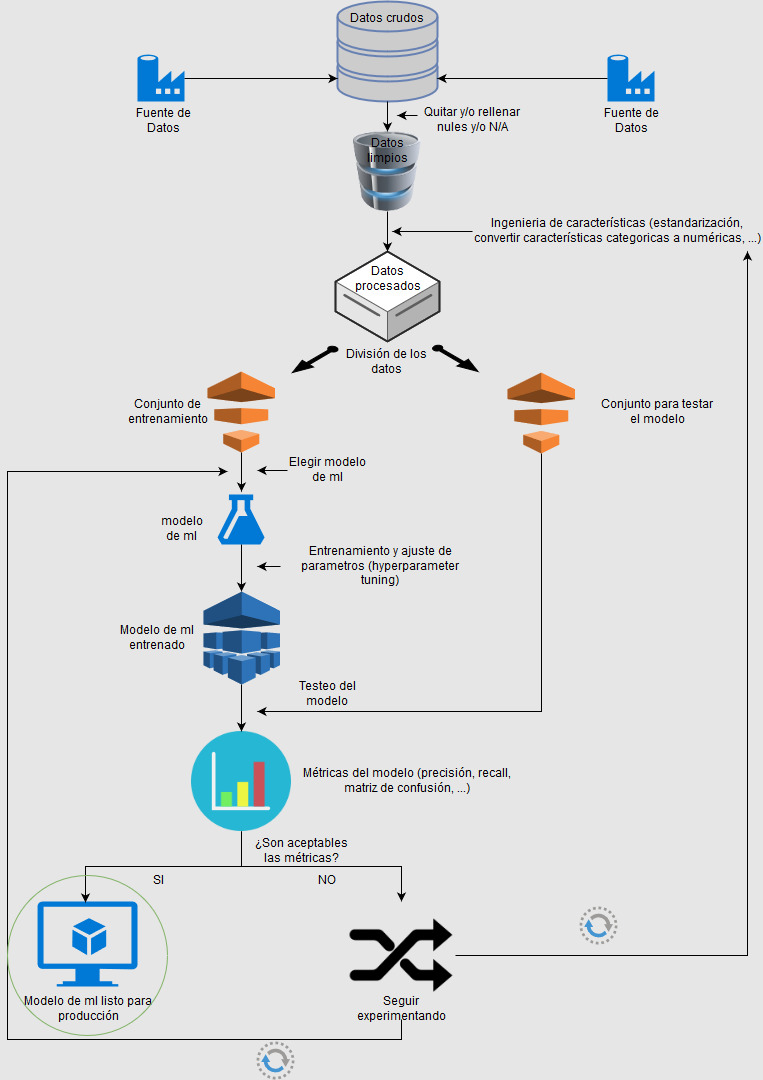
\includegraphics[width=\textwidth]{C:/Users/David/Desktop/TFG/TFGLatex/imagenes/ml_pipeline.jpg}
  \caption[\textit{Machine learning pipeline}]{Diagrama de flujo de un proyecto de \textit{machine learning}}
  \label{ml_pipeline}
\end{figure}

\clearpage


\chapter[Implementación paralela]{Implementación paralela de algoritmos}\label{chap:implementacion_paralela}
En este capítulo se implementarán algunos de los algoritmos mas populares de \textit{machine learning} 
pero con un enfoque distribuido, con el fin de minimizar los tiempos de ejecución a medida que
el \textit{dataset} se vuelve mas grande.
Cada sección consistirá en explicar de una manera breve y concisa la problemática a estudiar, 
el algoritmo a desarrollar, exponer el código fuente del algoritmo en paralelo y por último se mostrará
una gráfica comparativa de tiempos usando distintos enfoques para el mismo problema.
\newline

Para comenzar, vamos a establecer una serie de convenciones para la notación, con el fin de explicar
las matemáticas que hay detrás de los algoritmos de \textit{machine learning}.

El numero total de datos de entrenamiento se marcara con la letra $m$, mientras que es numero total
de características de los datos se denotara con la letra $n$.

Un dato de entrenamiento sera un vector fila donde cada componente del vector será una característica
de dicho dato. A cada dato del conjunto de entrenamiento se le denotara con la letra $x$ y un 
superíndice, mientras que las características se denotaran con la letra $x$ y subíndices. 

En caso de que el dato lleve aparejado una clase a la que pertenece, esta será denotada con la letra 
$y$. Así pues, para un primer ejemplo de entrenamiento (supervisado) sería:
$$ x^{(1)}=(\underbrace{x^{(1)}_1, x^{(1)}_2, \cdots, x^{(1)}_n}_{\text{n características}}); y^{(1)} $$

Al conjunto total de datos lo denotaremos con la letra $X$ que representará la matriz que contiene
todos los datos de entrenamiento, donde cada ejemplo será un vector fila de la matriz.
La letra $y$ será un vector columna conteniendo las clases de sus respectivos datos (aparejados por el índice), 
por lo que a la fila $i$-ésima de la matriz le corresponde la clase $i$-ésima del vector $y$.
Si estamos hablando de un problema de aprendizaje no supervisado, no tendría sentido hablar de las clases 
aparejadas a cada dato, con lo cual el vector $y$ no existiría.

A modo de ejemplo, el conjunto de entrenamiento para un problema de aprendizaje supervisado quedaría así:
%\vspace{1pt}

$$
X = \left(\begin{array}{ccc}
    \textemdash & x^{(1)} & \textemdash \\
    \textemdash & x^{(2)} & \textemdash \\
     & \vdots &  \\
    \textemdash & x^{(m)} & \textemdash \\
\end{array}\right)
%
=
  \left(\begin{array}{ccccc}
    x^{(1)}_1 & x^{(1)}_2 & x^{(1)}_3 & \cdots & x^{(1)}_n \\
    x^{(2)}_1 & x^{(2)}_2 & x^{(2)}_3 & \cdots & x^{(2)}_n \\
    \vdots & \vdots & \vdots & \ddots & \vdots \\
    x^{(m)}_1 & x^{(m)}_2 & x^{(m)}_3 & \cdots & x^{(m)}_n \\
\end{array}\right)
%
;
y = \left(\begin{array}{c}
    y^{(1)} \\
    y^{(2)} \\
    \vdots \\
    y^{(m)} \\
\end{array}\right)
$$

De manera análoga si hubiera que hacer distinción entre los datos de entrenamiento y los datos de test, 
se denotarán $X_{train}, y_{train}$ y $X_{test}, y_{test}$.


\section{Aprendizaje supervisado}
En el aprendizaje supervisado necesitamos que cada dato de entrenamiento lleve aparejado una clase 
a la que pertenece. De esta manera nuestro algoritmo intentara adaptarse a los datos lo mejor 
posible corrigiendo los errores en función de la clase real de cada ejemplo.
En esta sección se estudiaran los algoritmos de Regresión Lineal y \textit{NaiveBayes}.
\subsection{Regresión lineal}
La \textbf{Regresión Lineal}\index{Regresión!Lineal} es un potente algoritmo de \textit{machine learning} que 
permite predecir el comportamiento de una variable dependiente $y \in \mathds{R}$ a partir de los 
valores de la variable independiente $x \in \mathds{R}^n$.
El modelo se puede expresar como una ecuación o recta de regresión 
$$h_{\theta}(x) = \theta^T x = \theta_0 + \theta_1 x_1 + \cdots + \theta_n x_n$$
de la cual se debe ajustar el parámetro desconocido $\theta \in \mathds{R}^n$ para que el error 
de las predicciones sea el menor posible.

Dicho error viene representado por la función de perdida cuadrática
$$J(\theta) = \frac{1}{2m} \sum_{i=1}^{m}(\theta^Tx^{(i)} - y^{(i)})^2$$
donde $\theta^Tx^{(i)}$ representa el valor predecido para el ejemplo $i$-ésimo del \textit{dataset}, y la variable 
$y^{(i)}$ representa el valor real del ejemplo $i$-ésimo.

Gráficamente, en $\mathds{R}^2$, el problema consiste en ajustar lo mejor posible una recta a los 
puntos que representan los ejemplos de entrenamiento

\begin{figure}[h]
  \centering
  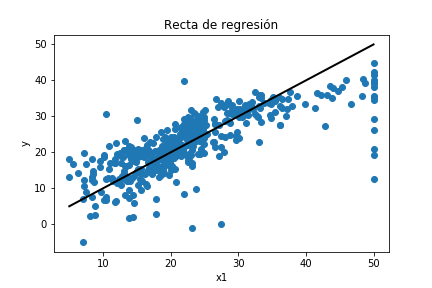
\includegraphics[width=\textwidth]{C:/Users/David/Desktop/TFG/TFGLatex/imagenes/recta_regresion.png}
  \caption[Regresión lineal en $\mathds{R}^2$]{Recta de regresión}
  \label{recta_regresion}
\end{figure}

\noindent \textbf{Gradiente de descenso}\\
Uno de los algoritmos mas populares de optimización de funciones es el algoritmo del Gradiente 
de Descenso\index{Gradiente de descenso} 
(\href{https://en.wikipedia.org/wiki/Gradient_descent}{\textit{Gradient Descent}}).
Este algoritmo consiste en actualizar los pesos o variables $\theta_i \enskip \forall i=1, \cdots, n$ de 
manera que con cada iteración se vaya reduciendo el error $J(\theta)$.
Las actualizaciones en cada iteración están dadas por la siguiente fórmula~\cite{DBLP:books/lib/Bishop07}

\begin{equation}
\theta := \theta - \alpha \frac{1}{m} \sum_{i=1}^{m}(h_{\theta}(x^{(i)}) - y^{(i)})x^{(i)}
\end{equation}

donde $\alpha$ es un parámetro que controla el salto que se produce en cada iteración del algoritmo, 
también denominado tasa de aprendizaje o \textit{learning rate}.
A valores pequeños del parámetro la iteración se vuelve mas lenta pero mas segura, por el contrario, 
valores grandes del parámetro producen que el algoritmo se acelere de manera considerable pero a costa 
de correr el riesgo de que incluso no llegue a converger.

\clearpage

Una manera lógica de paralelizar este computo es dividir el trabajo en el conjunto de entrenamiento 
de tal manera que cada máquina trabaje sobre un cierto numero de ejemplos de entrenamiento y no 
sobre el conjunto total.
Supongamos que nuestro conjunto de entrenamiento $X$ tiene un total de $m=4 \cdot 10^8$ de ejemplos.
Una iteración del algoritmo de descenso de gradiente tiene que recorrer todos los ejemplos y realizar 
un calculo con cada uno de ellos, sin embargo, definamos lo siguiente:
$$ temp^{(1)} = \sum_{i=1}^{10^8}(h_{\theta}(x^{(i)}) - y^{(i)})x^{(i)} $$
Este calculo sería realizado en una máquina (notese que solo utiliza un cuarto del \textit{dataset} original) 
de tal manera que esta máquina en particular solo contendría un cuarto del calculo total a realizar.
De manera análoga definimos
$$ temp^{(2)} = \sum_{i=10^8+1}^{2 \cdot 10^8}(h_{\theta}(x^{(i)}) - y^{(i)})x^{(i)} $$
que sería el calculo a realizar por la segunda máquina.
Así sucesivamente, hemos dividido el trabajo en 4 porciones que se desarrollan de manera totalmente 
independiente y paralela.\\
Sin embargo, el calculo de una iteración del gradiente de descenso no 
acaba aquí, ya que necesitamos combinar los resultados de estas cuatro máquinas.\\
Esto de nuevo en sencillo, ya que un ultimo cálculo requeriría juntar las cuatro porciones de la 
siguiente manera:
$$ \theta := \theta - \alpha \frac{1}{4 \cdot 10^8}(temp^{(1)} + temp^{(2)} + temp^{(3)} + temp^{(4)}) $$
De manera gráfica, para una paralelización en $n$ partes, cada partición de los datos se alojaría en un nodo
como un bloque de datos el cual sería procesado y luego enviado a través de la red a un nodo que recibiría
todas las partes y haría la agregación o combinación de los resultados.

\begin{figure}[h]
  \centering
  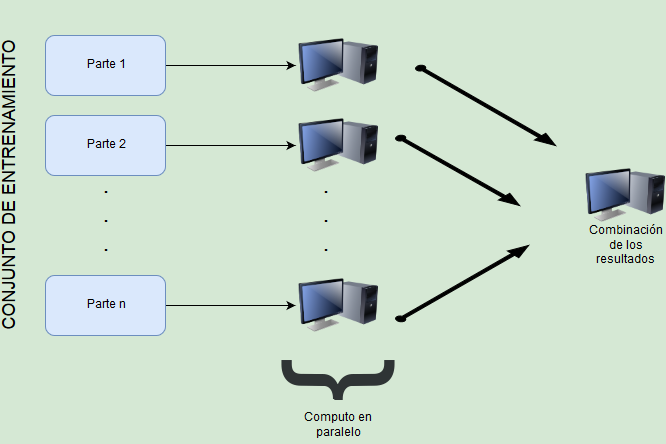
\includegraphics[width=\textwidth]{C:/Users/David/Desktop/TFG/TFGLatex/imagenes/computo_paralelo.png}
  \caption[División de los datos en el gradiente de descenso]
          {Computo en paralelo y agregación de los datos}
  \label{computo_paralelo}
\end{figure}

\newpage

\subsubsection*{Código \textit{Spark} Regresión lineal}
\lstinputlisting[caption=LinearRegression.py, language=Python, firstline=8]
                {C:/Users/David/Desktop/TFG/implementaciones/LinearRegression.py}

\begin{lstlisting}[language=bash, numbers=none]
$ spark-submit --master yarn-client LinearRegression.py
\end{lstlisting}

\clearpage

\subsection{Naive-Bayes}
Un clasificador \textbf{NaiveBayes}\index{NaiveBayes} es un clasificador probabilístico que se apoya en el 
\textit{Teorema de Bayes} para clasificar las entradas.
Es un modelo que asume que las características de las variables de entrada son independientes 
entre sí, esto es, el valor de una cierta variable no influye para nada en el valor de otra.\\
La idea general detrás del algoritmo es calcular la media y la varianza de cada clase y cada característica.
Una vez realizado ésto, se pueden utilizar los valores obtenidos para predecir la clase de un nuevo 
dato de entrada. El modelo lo etiquetará con la clase que mas se parezca de las vistas en el 
conjunto de entrenamiento.
\newline

Como se ha mencionado anteriormente, el algoritmo utiliza el teorema de Bayes para asignar la probabilidad de
un suceso condicionado a la ocurrencia de otro. En el ejemplo explicado mas abajo dichos sucesos serían la
probabilidad a priori y a posteriori de ser hombre o mujer.
%\newline

\begin{theorem}[Teorema de Bayes]\index{Teorema de Bayes}
  Sean ${A_1, A_2, \cdots, A_n}$ sucesos con $P(A_i) \neq 0 \quad \forall i=1, 2, \cdots, n$. 
  Sea $B$ un suceso cualquiera del que se conocen $P(B|A_i) \quad \forall i=1, 2, \cdots, n$.
  Entonces:
  {\fboxsep 8pt\fboxrule 1pt
  \begin{equation*}
  \fbox{$ P(A_i|B) = \frac{P(B|A_i) \cdot P(A_i)}{P(B)} $}
  \end{equation*}
  }
%  $$ P(A_i|B) = \frac{P(B|A_i) \cdot P(A_i)}{P(B) $$
\end{theorem}

Supongamos que queremos clasificar a una persona en hombre o mujer a través de características como 
la altura, el peso y el numero de pie. Aquí nuestras características serian $n=3$ y el objetivo 
sería predecir la variable $y=0$ si es hombre o $y=1$ si es mujer.
A partir de un \textit{dataset} de ejemplos etiquetados con hombre o mujer,
el concepto de aprendizaje para el algoritmo  sería calcular la media y la varianza 
de la altura, el peso y la talla de pie de todos los hombres y mujeres por separado.
Con estos datos, estamos en disposición de calcular la probabilidad a posteriori y las probabilidades 
condicionadas que servirán al algoritmo para realizar sus predicciones.

\begin{figure}[!htpb]
  \centering
  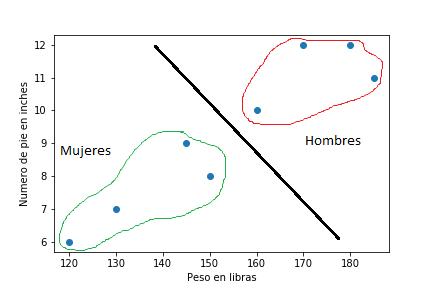
\includegraphics[width=0.5\textwidth]{C:/Users/David/Desktop/TFG/TFGLatex/imagenes/naiveBayes_men_women.png}
  \caption[Naive Bayes clasificación]{Clasificación entre hombres y mujeres}
  \label{men_women_boundary}
\end{figure}

Debido a la simplicidad de los cálculos que usa para entrenarse, \textit{NaiveBayes} se desempeña muy bien 
en conjuntos de datos muy grandes dando lugar a modelos muy precisos.\\
Sin embargo, como todo modelo, tiene sus ventajas e inconvenientes que hacen de \textit{NaiveBayes} un modelo 
propicio para unos determinados tipos de problemas.

\begin{itemize}
  \item Ventajas:
  \begin{enumerate}
    \item Funciona muy bien en problemas multiclase. Dado un dato, es rápido y fácil predecir su clase.
    \item Asumiendo la independencia de las clases, un clasificador \textit{NaiveBayes} obtiene un mejor 
    desempeño comparado con otros métodos como la regresión logística, además necesita menos datos 
    de entrenamiento.
  \end{enumerate}
  \item Inconvenientes:
  \begin{enumerate}
    \item Si en los datos de test hay una característica nunca antes vista en los datos de 
    entrenamiento, el modelo le asignará una probabilidad de 0 y será incapaz de hacer una predicción.
    Esto es conocido como frecuencia cero o \textit{zero frequency}.
    \item En la vida real, es casi imposible encontrar un \textit{dataset} donde todas las características 
    sean completamente independientes unas de las otras.
  \end{enumerate}
\end{itemize}

\subsubsection*{Código MapReduce NaiveBayes}
\lstinputlisting[caption=NaiveBayes.py, language=Python, firstline=10]
                {C:/Users/David/Desktop/TFG/implementaciones/NaiveBayes.py}
                  
\begin{lstlisting}[language=bash, numbers=none]
$ python NaiveBayes.py <input_file> [-r hadoop]
\end{lstlisting}

Para el desarrollo de este código se ha elegido el \textit{framework MapReduce} debido a que la arquitectura del
algoritmo es altamente paralelizable, esto es consecuencia de la asociatividad de las operaciones que se calculan.\\
En la fase \textit{map} se parsea la línea y se separa en campos (divididos por coma), las características se 
asignan a la variable $x$ y el último campo es la clase, asignada a la variable $y$.\\
Como clave se emite una tupla que tiene por valor la clase ($y$) y la posición del campo ($i$), mientras que
como valor se emite otra tupla que contiene el valor del propio campo ($x[i]$) y un 1 que servirá para hacer
un conteo de los datos. Esta elección ha sido así ya que se consigue la máxima paralelización al dividir las 
claves (\textit{key}) en tantas como campos tengan los registros.\\
En la fase \textit{reduce} se crean 3 variables: $m$, $sum\_features$ y $sum\_features\_squared$. La primera sirve
para hacer la agregación del conteo de registros, la segunda y tercera sirven como variables auxiliares para 
posteriormente calcular la media $\mu_j$ y la varianza $\sigma^2$.
                    
\clearpage


\section{Aprendizaje no supervisado}
En el aprendizaje no supervisado es el propio algoritmo el que debe sacar los patrones de 
comportamiento de todo el conjunto de datos.
En esta sección se estudiaran los algoritmos de Detección de anomalías y \textit{K-Means}.
\subsection{Sistema de detección de anomalías}
Un sistema de detección de anomalías es un software capaz de detectar comportamientos anómalos a 
partir de comportamientos previamente establecidos como normales.
La base de este modelo es la distribución Gaussiana y requiere que nuestro conjunto de 
datos tenga variables o características que se distribuyan según una normal de media $\mu$ y  
varianza $\sigma^2$, es decir, $\mathcal{N}(\mu, \sigma^2)$.\\
Este modelo es usado frecuentemente en detección de intrusos de una red, monitorización de las 
máquina de un data center, detección de fraude en el uso de tarjetas de crédito...
\newline

La distribución Gaussiana\index{Distribución!Gaussiana} (o distribución normal\index{Distribución!Normal}) 
es una distribución de probabilidad que aparece con mucha frecuencia en fenómenos reales, lo cual es ideal 
para poder modelar estos fenómenos desde un punto de vista estadístico.

\begin{figure}[h]
  \centering
  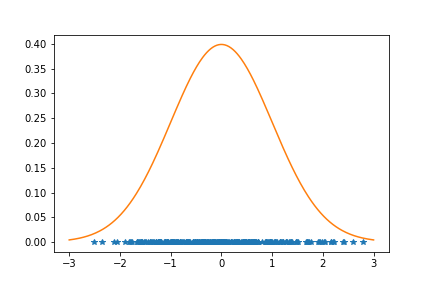
\includegraphics[scale=0.6]{C:/Users/David/Desktop/TFG/TFGLatex/imagenes/normal_01.png}
  \caption[$\mathcal{N}(0,1)$]{Distribución normal de media 0 y desviación típica 1}
  \label{normal_01}
\end{figure}

Esta función será nuestro punto de partida para construir nuestro modelo, el cual asume que las 
características de los datos siguen dicha distribución, es decir, 
$\forall j=1,\cdots,n; \quad x_j \sim \mathcal{N}(\mu_j, \sigma_j^2)$.\\

El objetivo es modelizar una función que denotaremos $p(x)$, la cual, dado un ejemplo nos devuelva la 
probabilidad de que dicho ejemplo sea anómalo. Más adelante se definirá esta función de manera 
concreta.\\
Lo primero que debemos hacer es calcular las medias y varianzas de cada característica de nuestros 
ejemplos de entrenamiento (matriz $X$), esto nos da una serie de parámetros 
$\mu = (\mu_1, \ldots, \mu_n) $ y 
$\sigma^2 = (\sigma_1^2, \ldots, \sigma_n^2) $ 
que se utilizaran posteriormente para predecir la probabilidad de que un nuevo dato sea anómalo. 
Más concretamente:
$$ \mu_j = \frac{1}{m}\sum_{i=1}^{m}x_j^{(i)} \quad 
   \sigma_j^2 = \frac{1}{m}\sum_{i=1}^{m}(x_j^{(i)} - \mu_j)^2 $$

\noindent Una vez que tenemos nuestros parámetros calculados ya podemos definir $p(x;\mu,\sigma^2)$ como:
$$ p(x;\mu,\sigma^2) = \frac{1}{\sqrt{2\pi}\sigma}e^{-\frac{1}{2}\frac{x-\mu}{\sigma^2}^2}$$
Esta fórmula nos da la probabilidad de que un valor de una determinada característica se 
comporte de manera anómala.

\clearpage

Una vez calculadas todas las curvas gaussianas para cada característica del \textit{dataset}, definimos $p(x)$ como:
$$ p(x) = \prod_{j=1}^n p(x_j;\mu_j,\sigma_j^2)= p(x_1; \mu_1, \sigma_1^2) \cdots  p(x_n; \mu_n, \sigma_n^2)$$
La función $p(x)$ se comporta como un detector de irregularidades ya que si alguna de las funciones 
$p(x_j;\mu_j,\sigma_j^2)$ para cierto $j$ arroja un valor fuera de lo normal, este quedará reflejado 
en el valor final de $p(x)$.\\
Llegados a este punto, debemos establecer un cierto umbral $\epsilon$ que nos marque la frontera 
para considerar un ejemplo como normal o anómalo, es decir, marcaremos un ejemplo $x$ como anómalo si 
$p(x)<\epsilon$ y será considerado normal si por el contrario $p(x)>=\epsilon$.
Esta elección del parámetro $\epsilon$ no es algo universal sino que depende del problema en cuestión 
(\autoref{circles_plot}) y el \textit{dataset} utilizado para modelar $p(x)$.
Existen ciertas directrices así como reglas generales para una buena elección de 
$\epsilon$\footnote{\url{https://www.coursera.org/learn/machine-learning/lecture/Mwrni/developing-and-evaluating-an-anomaly-detection-system}}, pero están fuera de los objetivos de este documento.
\newline
Gráficamente, la función $p(x)$ establece una bola n-dimensional con un cierto centro 
y radio que dependerá del epsilon elegido y el \textit{dataset} utilizado. Toda representación 
de un ejemplo en el espacio $\mathds{R}^n$ que quede dentro de dicha bola, será considerado normal, 
si por el contrario dicha representación queda fuera de la bola, entonces será considerado una 
anomalía.

\begin{figure}[h]
  \centering
  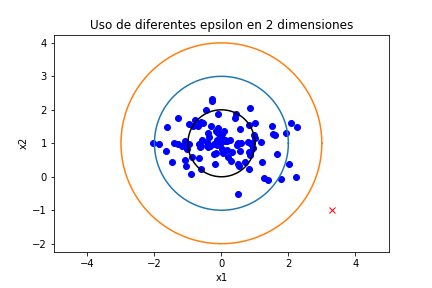
\includegraphics[scale=0.6]{C:/Users/David/Desktop/TFG/TFGLatex/imagenes/circles_plot.png}
  \caption[Ejemplo de anomalía]{Ejemplo de anomalías para distintos valores de $\epsilon$}
  \label{circles_plot}
\end{figure}

En la figura los valores se distribuyen según
$x1 \sim \mathcal{N}(0, 1); \quad x2 \sim \mathcal{N}(1, 0.5)$.
Los círculos concéntricos representan la elección de distintos valores del parámetro $\epsilon$ ,
centrados en el punto $\mu=(\mu_1, \mu_2)=(0, 1)$.
Si tomamos como referencia el circulo más grande, la $x$ marcada en rojo sería un ejemplo anómalo 
en ese conjunto de datos

\newpage  
  
\subsubsection*{Código MapReduce para el computo de la media y la varianza}
  
\lstinputlisting[caption=ComputeMeanVar.py, language=Python, firstline=10]
                {C:/Users/David/Desktop/TFG/implementaciones/ComputeMeanVar.py}

\begin{lstlisting}[language=bash, numbers=none]
$ python ComputeMeanVar.py <input_file> [-r hadoop]
\end{lstlisting}

La elección de \textit{MapReduce} para desarrollar este algoritmo ha sido debido a que para calcular la media y 
la varianza de un conjunto de datos, solo es necesario un escaneo completo del \textit{dataset}. Como se ve
gráficamente en la \autoref{mapReduce_wordcount}, en la fase map se produce el parseo de los datos donde cada línea
se divide separando los campos por coma (\textit{,}). Los valores emitidos son: la posición del campo ($i$) como clave
y el valor del campo ($fields[i]$) y un 1 como valor. Este 1 sirve para hacer un conteo de los datos en la fase 
\textit{reduce}.\\
En dicha fase \textit{reduce}, se itera sobre los valores recibidos en la fase \textit{map} y se descompone el calculo
de la media en 2 variables, aparte de crear otra variable $m$ que será un contador de los registros totales por cada campo.
Una vez terminado la iteración del \textit{for}, se utilizan las variables \textit{sum\_features} y 
\textit{sum\_features\_squared} para calcular la media $\mu_j$ y la varianza $\sigma^2$.
\newline

Para el despliegue de la aplicación, se puede hacer de manera local (usado principalmente para depuración del código)
o de manera distribuida haciendo uso de un \textit{cluster Hadoop} para que la computación se produzca en paralelo
(\textit{-r hadoop}). Este último modo de despliegue sube el archivo \path{input_file} a \textit{HDFS} para su 
posterior ejecución con \textit{MapReduce}. También se puede indicar que el archivo ya se encuentra en \textit{HDFS}
poniendo delante el prefijo de hdfs en el path: \path{hdfs://<input_file_in_hdfs>}
  
\newpage

\subsection{K-Means}
\textbf{\textit{K-Means}}\index{K-Means} es uno de los algoritmos de \textit{clusterización}\index{Clusterización} más 
extendidos y usados en la actualidad. La idea principal del algoritmo es agrupar los datos de entrada 
en distintos conjuntos o \textit{clusters}\footnote{Notese que no se debe confundir el uso de la 
palabra \textit{cluster} para hacer referencia a un \textit{cluster} de maquinas, o cuando se usa 
para referirnos a un conjunto de datos agrupados.} 
coherentes, esto es, los puntos dentro de una mismo \textit{cluster} son más parecidos entre sí 
que los puntos de otro \textit{cluster} cualquiera.
\newline

Nuestros datos de entrada son puntos $x^{(i)} \in \mathds{R}^n$ y un cierto numero $k \in \mathds{N}$ de 
\textit{clusters} en los que vamos a agrupar nuestros datos.\\
Comenzamos estableciendo $k$ puntos en lugares aleatorios de nuestros datos, estos puntos serán los 
centros de los \textit{clusters} $c_1, c_2, \cdots, c_k$, y los llamaremos \textit{centroides}\index{Centroides}.
Una vez hecho esto, el algoritmo recorrerá cada punto $x_i$ y encontrará el centroide $c_j$ más 
cercano (en términos de la distancia euclídea) a nuestro punto. Por lo cual, al punto $x_i$ se le 
asigna el \textit{cluster} $j$.\\
Una vez que tengamos todos los puntos asignados a sus respectivos centroides más cercanos, actualizamos 
los centroides con la media de todos los puntos que pertenecen al \textit{cluster} de dicho centroide.\\
Las iteraciones del algoritmo se detendrán cuando en dos iteraciones sucesivas ninguno de los puntos 
sea asignado a otro \textit{cluster} distinto al anterior o cuando la norma del vector que componen 
la resta de los centroides de dos iteraciones consecutivas sea menos que un cierto $\epsilon$ 
prefijado.
\newline

\noindent \textbf{Pasos del algoritmo K-Means}:
\begin{enumerate}
  \item[] \textbf{Input}: Puntos en $\mathds{R}^n$ y un numero $k \in \mathds{N}$ de \textit{clusters}
  en los que agrupar nuestros datos.
  \item Insertar $k$ centroides $c_1, c_2, \cdots, c_k$ en localizaciones aleatorias.
  \item Calcular la distancia entre cada punto $x^{(i)}$ y cada centroide $c_i$.
  \item Asignar a cada punto $x^{(i)}$ al \textit{cluster} cuya distancia al centroide sea menor 
        que la distancia al resto de centroides.
  \item Recalcular los nuevos centroides usando la formula $c_i = \frac{1}{m_j} \sum_{j=1}^{m_i}x^{(i)}$ 
        donde $m_i$ es el número de puntos que pertenecen al \textit{cluster} $i$ y $x^{(i)}$ son 
        todos los puntos de dicho cluster, más concretamente \\
        $x^{(i)} \in \{ p \in \mathds{R}^n \, | \, d(p, c_j) < d(p, c_s) \, \forall s \in 1, \cdots, k; s \neq j \}$.
  \item Calcular la norma entre los centroides anteriores y los nuevos centroides \\
        $ ||(c_1^i, c_2^i, \cdots, c_k^i) - (c_1^{i-1}, c_2^{i-1}, \cdots, c_k^{i-1})||_{\infty} $ 
        donde el superíndice $i$ indica la iteración $i$-ésima.
  \item Si dicha norma es menor que un cierto $\epsilon$ prefijado entonces parar (se ha llegado a la convergencia), 
        en caso contrario volver al paso $2$.
  \item[] \textbf{Output}: $k$ centroides $c_1, c_2, \cdots, c_k$.
\end{enumerate}

\begin{figure}[htp]
  \centering
  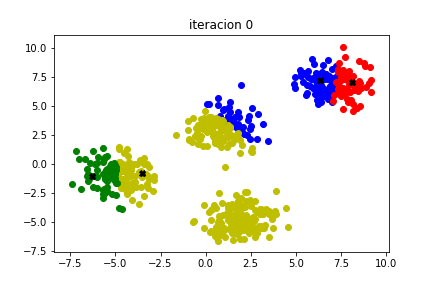
\includegraphics[width=.3\textwidth]{C:/Users/David/Desktop/TFG/TFGLatex/imagenes/kmeans_imagen0.png}\quad
  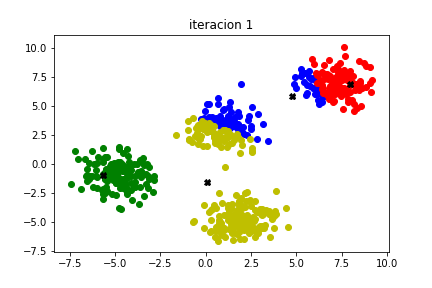
\includegraphics[width=.3\textwidth]{C:/Users/David/Desktop/TFG/TFGLatex/imagenes/kmeans_imagen1.png}\quad
  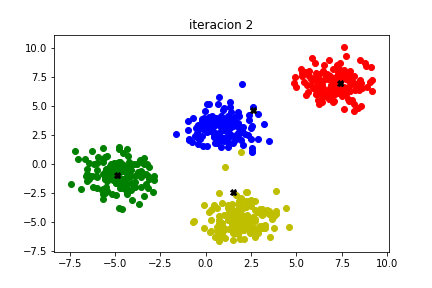
\includegraphics[width=.3\textwidth]{C:/Users/David/Desktop/TFG/TFGLatex/imagenes/kmeans_imagen2.png}

  \medskip

  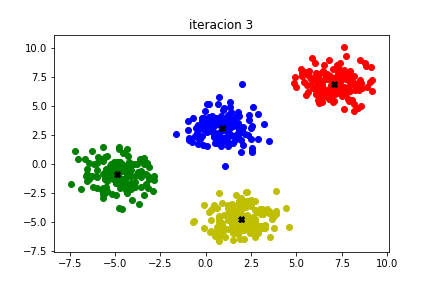
\includegraphics[width=.3\textwidth]{C:/Users/David/Desktop/TFG/TFGLatex/imagenes/kmeans_imagen3.png}\quad
  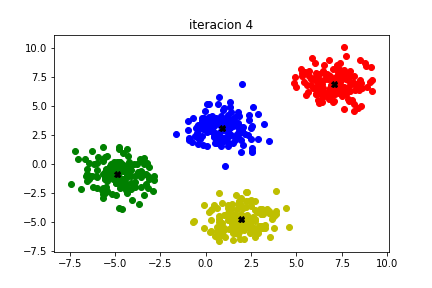
\includegraphics[width=.3\textwidth]{C:/Users/David/Desktop/TFG/TFGLatex/imagenes/kmeans_imagen4.png}

  \caption{Iteraciones del algoritmo k-means}
  \label{kmeans_iteraciones} % para las hyperreferencias
\end{figure}

\newpage

\subsubsection*{Código \textit{Spark} para el algoritmo de \textit{K-Means}}

\lstinputlisting[caption=KMeansSpark.py, language=Python, firstline=8, lastline=72]
                {C:/Users/David/Desktop/TFG/implementaciones/KMeansSpark.py}

\clearpage
Con el fin de testar el código anteriormente escrito:

\lstinputlisting[caption=KMeansMain, language=Python, firstline=74]
                {C:/Users/David/Desktop/TFG/implementaciones/KMeansSpark.py}

\begin{lstlisting}[language=bash, numbers=none]
$ # master puede ser local[*] o yarn-client
$ spark-submit --master yarn-client KMeansSpark.py
\end{lstlisting}

Para el desarrollo de este código se ha elegido el \textit{framework Spark} debido principalmente a que el algoritmo
de \textit{K-Means} es un algoritmo iterativo sobre los mismos datos para realizar los computos. Debiado a la capacidad
de \textit{Spark} de cachear los datos en memoria, los tiempos de ejecución se reducirán considerablemente.
\newline

Los datos de entrada del algoritmo es un \textit{RDD} que contiene como registros objetos \textit{numpy arrays}.
Lo primero que se hace es cachear los datos en memoria y a continuación inicializar los centroides en posiciones
aleatoria de los datos de entrada.\\
Dentro del bucle \textit{while}, la variable \textit{points\_clusterized} contiene un mapeo de los datos originales
a una tupla que contiene el centroide más cercano al punto $p$ en cuestión y un 1 que permite realizar posteriormente
el conteo de los puntos totales. La variable \textit{clusters\_set} realiza una agregación que suma los puntos de
entrada y los unos anteriores para realizar la media de cada \textit{cluster} de puntos.\\
La variable \textit{new\_centroids} realiza un mapeo de los valores para calcular la división 
de la suma de los puntos y el conteo, de esta manera se obtienen los nuevos centroides que se guardan en la variable
\textit{new\_centroids}. Por último, se calcula la distancia entre los nuevos centroides y los anteriores con el fin
de calcular la distancia para el criterio de parada (del bucle \textit{while}).\\
Las iteraciones se detendrán cuando la distancia entre los centroides de dos iteraciones consecutivas sea menor
que un cierto $\epsilon$ prefijado (o cuando se superen las máximas iteraciones permitidas).
\newline

El modo de despliegue de la aplicación depende de si como \textit{master} ponemos que se ejecute en local 
(\textit{local[*]}) o en distribuido (\textit{yarn-client}). El primero no distribuye ningún cálculo en absoluto
mientras que el segundo es un cliente del gestor de recursos del \textit{cluster}, \textit{YARN}.

\newpage


%%%%%%%%%%%%%%%%%%%%%%%%%%%%%%%%%%%%%%%%%%%%%%%%%%%%%%%%%%%%%%%%%%
%%%%%%%%%%%%%%%%%%%%%%% CONCLUSION %%%%%%%%%%%%%%%%%%%%%%%%%%%%%%%
%%%%%%%%%%%%%%%%%%%%%%%%%%%%%%%%%%%%%%%%%%%%%%%%%%%%%%%%%%%%%%%%%%

\chapter*{Conclusión y líneas de trabajo futuras}
\addcontentsline{toc}{chapter}{Conclusión}
\markboth{Conclusión}{} % para que la cabecera coincida bien con el capítulo
% Mini mini resumen del report
Hemos visto como desplegar un \textit{cluster} de máquinas utilizando el software  \textit{Apache Hadoop}, 
y posteriormente utilizarlo para desarrollar algoritmos paralelos de \textit{machine learning}. Dichos algoritmos
se han desarrollado tanto en \textit{MapReduce} como en \textit{Spark}.

Respecto a los conocimientos necesarios para abordar este trabajo, del grado en \textbf{Ciencias Matemáticas}
cabe destacar por su especial utilidad las asignaturas de programación paralela, geometría computacional y 
programación declarativa entre otras. Todas ellas pertenecientes al itinerario de \textbf{ciencias de la computación}.
Adicionalmente a estos conocimientos, también han sido especialmente necesario aprender el funcionamiento
de los sistemas \textit{UNIX} (en particular de \textit{LINUX}), sobre todo su uso a través de la línea de comandos 
(\textit{CLI}, \textit{Command Line Interface}). 
Si bien no hay una asignatura específica para aprender estos sistemas operativos en la carrera de Matemáticas, 
el libro \cite{unix_programming_environment} es un buen punto de partida para comenzar.
%%%%%%%%%%%%%%%%%%%%%%%%%%%%%%%

% Retomar los objetivos y evaluarlos
\subsection*{Evaluación de los objetivos}
Los objetivos expuestos en la sección de \nameref{objetivos_plan_trabajo} 
se han realizado siguiendo el plan de trabajo establecido. A modo de evaluación vamos a repasarlos:

\begin{itemize}
  \item Instalación de un \textbf{\textit{cluster Hadoop}} de máquinas virtuales.
  \begin{itemize}
    \item[] El despliegue del \textit{cluster} se ha realizado sobre máquinas virtuales usando \textit{Cloudera Manager}
            como herramienta principal. En la \autoref{test_cluster_desplegado} se comprobó como la instalación
            se realizó correctamente y todos los servicios desplegados (\textit{HDFS}, \textit{YARN}...) funcionaban bien.\\
            En esta parte la mayor dificultad radica en la instalación de todos los componentes que necesita 
            \textit{Hadoop} para su correcto funcionamiento, es decir, \textit{Java}, \textit{MySQL}, \textit{NTP}...\\
            Como \textit{Cloudera Manager} es un asistente gráfico, facilita enormemente el trabajo que va por detrás
            ya que lo gestiona automáticamente. Sin embargo, para realizar dicho despliegue conviene tener muy clara
            la teoría detrás de los servicios de \textit{Hadoop}, donde viene muy bien explicada en el libro 
            \cite{White:2009:HDG:1717298}.\\
            Respecto a los \textit{frameworks} de procesamiento que hemos instalado, el proceso ha sido bastante sencillo
            debido a las herramientas de \textit{Cloudera} y al gestor de paquetes de \textit{Python}. Esta parte no
            supuso mayor complicación.
  \end{itemize}
  \item Desarrollo de algoritmos de \textbf{\textit{machine learning}} de manera paralela.
  \begin{itemize}
    \item[] Los algoritmos desarrollados cumplen con las características que todo algoritmo distribuido debe cumplir,
            especialmente en lo que se refiere a la \textbf{escalabilidad}. El incremento de los datos a procesar solo
            penaliza el rendimiento en cuanto a tiempo de ejecución y nunca llega a colapsar el programa. 
            Tanto los algoritmos desarrollados en \textit{MapReduce} como en \textit{Spark} cumplen con dichas 
            condiciones de escalabilidad si bien el diseño de cada uno de ellos es diferente debido a su 
            arquitectura interna.\\
            La clave a la hora de conseguir este objetivo es tener en mente que el diseño de los algoritmos paralelos
            se basa en no guardar variables en memoria que puedan colapsar la capacidad del nodo trabajador.
            El proceso de desarrollo de algoritmos distribuidos implica cambiar la mentalidad a la hora de escribir
            el código ya que los datos se encuentran repartidos en distintas máquinas que funcionan de manera 
            asíncrona. El reto en este objetivo era desarrollar estos algoritmos en lo que a buenas prácticas se refiere.
  \end{itemize} 
\end{itemize}

\clearpage

\subsection*{Líneas de trabajo futuras}
Este proyecto puede servir como base para futuros trabajos relacionados con los temas que aquí se tratan, 
entiendase \textit{Big Data}, \textit{Machine Learning}, \textit{Apache Hadoop}, \textit{Apache Spark}...\\
Como primera línea de trabajo futuro se puede relacionar con temas de \textbf{\textit{Deep Learning}}\index{Deep Learning}, que es una rama encuadrada dentro del \textit{machine learning} 
y está enfocada en las redes neuronales convolucionales, que por su naturaleza estas toman un gran 
tiempo de entrenamiento.\\
Dentro del \textit{deep learning}, se puede avanzar en el estudio y desarrollo de técnicas paralelas para poder
entrenar redes neuronales convolucionales (\textit{CNN} por sus siglas en inglés) en un \textit{cluster} 
y así reducir los tiempos de ejecución.
En la tabla \autoref{MachineLearningVSDeepLearning} se muestran las principales diferencias conceptuales
entre \textit{machine learning} y \textit{deep learning}.

\begin{table}[!htpb]
  \centering
  \begin{tabular}{|r|c|c|} % tabla
    \hline
    & \textbf{\textit{Machine Learning}} & \textbf{\textit{Deep Learning}} \\ \hline
    Conjunto de entrenamiento & medio & grande \\ \hline
    Ingeniería de características & manual & automática \\ \hline
    Clasificadores disponibles & muchos & pocos \\ \hline
    Tiempo de entrenamiento & medio & grande \\ \hline
  \end{tabular}
   \caption[Diferencias entre \textit{Machine Learning} y \textit{Deep Learning}]
           {Diferencias entre \textit{Machine Learning} y \textit{Deep Learning}}
   \label{MachineLearningVSDeepLearning}
\end{table}

Otra posible línea de investigación reside en el uso de \textbf{\textit{GPU}}\footnote{Graphic Procesing 
Unit}\index{GPU} para la aceleración del proceso de entrenamiento de una red neuronal, y en concreto 
de una \textit{CNN}\footnote{Convolutional Neural Network}. 
Este proceso paralelo se puede ejecutar bien sea en una solo máquina (como puede ser un ordenador personal) 
o bien en un \textit{cluster} de máquinas donde cada nodo lleve incorporado una Unidad de Procesamiento Gráfico. \\
Los procesadores gráficos de \href{http://www.nvidia.es/page/home.html}{\textit{NVIDIA}} poseen una 
arquitectura de cálculo paralela llamada \href{http://www.nvidia.es/object/cuda-parallel-computing-es.html}{\textit{CUDA}}
(\url{http://www.nvidia.es/object/cuda-parallel-computing-es.html})
 que permite aprovechar dicha tarjeta gráfica para realizar cómputos. Es especialmente útil en la multiplicación 
de matrices ya que esencialmente una red neuronal se compone de matrices distinguidas en varias capas.
Este trabajo puede servir de base para futuros proyectos acerca de la utilización de \textit{GPU's} en 
\textit{clusters} de máquinas.
\newline

Una tercera línea de investigación posible es la utilización de algoritmos para otros fines de los que
inicialmente fueron destinados. Para la compresión de imágenes se pueden utilizar distintos algoritmos de
\textit{machine learning} como por ejemplo \textit{KMeans} o \textit{PCA}\index{PCA}
\footnote{\textit{Principal Component Analysis}} (\cite{DBLP:books/lib/HastieTF09}).\\
Un tipo especial de redes neuronales denominadas autocodificadores o \textit{autoencoders} son aquellas que
tienen 3 capas (una de entrada, una oculta y otra de salida) donde la capa de entrada y de salida son la misma
y la capa oculta posee menos neuronas que las otras dos para así obligar a la red que aprenda a codificar los
datos de entrada en un formato mas comprimido.

%%%%%%%%%%%%%%%%%%%%%%%%%%%%%

\clearpage



%%%%%%%%%%%%%%%%%%%%%%%%%%%%%%%%%%%%%%%%%%%%%%%%%%%%%%%%%%%%%%%%%%
%%%%%%%%%%%%%%%%%%%%%%% APENDICE %%%%%%%%%%%%%%%%%%%%%%%%%%%%%%%%%
%%%%%%%%%%%%%%%%%%%%%%%%%%%%%%%%%%%%%%%%%%%%%%%%%%%%%%%%%%%%%%%%%%

\part{Apéndice}\label{part:apendice}
\appendix
\chapter{Kaggle y KDD}
\textbf{Kaggle}\index{Kaggle} es una plataforma que aloja datos de diversas fuentes y organiza 
competiciones para que todo aquel que desee pueda desarrollar sus modelos predictivos y analíticos 
con el objetivo de conseguir el mayor desempeño.
Esta página pone en contacto diversos perfiles de personas (científicos de datos, mineros de datos...) 
con diversos problemas que a menudo exponen compañías y premian a aquellos equipos de personas que 
obtengan la mejor puntuación.
La plataforma tiene una serie de conceptos sobre los que se desarrolla:
\begin{description}
  \item[Competiciones] Permite a las empresas ponerse en contacto con los científicos de datos de la 
  comunidad Kaggle para resolver determinados problemas para su propio beneficio. Los mejores equipos 
  reciben una compensación económica así como puntos para el ranking interno de Kaggle.
  Las competiciones están clasificadas por nivel de dificultad, variando desde un nivel principiante 
  para iniciarse en el mundo de la ciencia de datos hasta un nivel experto en el cual obliga a los 
  participantes a desarrollar un proyecto de \textit{machine learning} de inicio a final (\textit{end to end}), esto es, 
  preprocesamiento, ingeniería de características, elección del modelo, evaluación...
  \item[Datasets] La plataforma aloja datos de muy diversas fuentes a disposición de todo aquel que quiera usarlos
  para entrenar sus modelos de \textit{machine learning}. Nos encontramos con datos que van desde clasificación o
  regresión hasta clusterización.
  \item[Kernels\index{Kernels}] Los kernels en Kaggle son \textit{scripts} de código que pueden ser ejecutados 
  en la nube y sirven de ayuda al resto de la comunidad para iniciarse en un cierto problema, preprocesar un 
  conjunto de datos, construir un modelo...
  Los kernels permiten ser valorados por el resto de usuarios que pueden premiar tu trabajo con votos y comentarios.
\end{description}
Además de todo lo mencionado anteriormente, Kaggle dispone de un foro para discutir las diversas 
problemáticas que puedan surgir a cada usuario. Conecta a miles de \textit{Data Scientish} de todo el mundo 
para que intercambien ideas y conocimientos.
La plataforma fue fundada por \href{https://en.wikipedia.org/wiki/Anthony_Goldbloom}{Anthony Goldbloom} 
en el año 2010 y se puede acceder a través de \url{https://www.kaggle.com/}
\newline

\vspace*{1cm}

\noindent\textbf{KDD}\index{KDD} viene de sus siglas en inglés \textit{Knowledge Discover Dataset}, y se refiere al hecho 
de sacar información útil de un \textit{dataset}, es decir, extraer conocimiento de los datos.
En su página web \url{http://www.kdd.org/} podemos encontrar toda la información relacionada con lo 
que hacen y a que se dedican. Organizan conferencias y eventos acerca de \textit{KDD}, 
publican \textit{papers}\footnote{documentos que contienen trabajos científicos}
y noticias acerca de temas de innovación, investigaciones y demás temas en relación con el \textit{KDD}.
Cada año lanza una competición abierta al público para que todo aquel interesado pueda descargarse 
el conjunto de datos que proporciona y realizar la tarea que se busca. Una de las \textit{KDD Cup} más famosas 
fue la del año 1999 \url{http://kdd.ics.uci.edu/databases/kddcup99/kddcup99.html}.
\newline

\vfill

\noindent \textbf{Algunos repositorios de \textit{datasets} de interés:}\\
\url{https://www.kaggle.com/datasets}\\
\url{http://archive.ics.uci.edu/ml/index.php}\\
\url{http://deeplearning.net/datasets/}\\


\chapter{Cloudera}\label{apendix:cloudera}
\textbf{\textit{Cloudera}}\index{Cloudera} es una compañía que proporciona software basado en 
\textit{Apache Hadoop}, formación y soporte técnico. 
De dicho software, en este trabajo se ha usado \textit{Cloudera Manager}, aquí se explica de manera general 
las 2 posibles opciones para desplegar un \textit{cluster}
\begin{itemize}
  \item \textit{CDH} (\textit{Cloudera Distribution Hadoop})\index{Cloudera!CDH} es una distribución de 
  \textit{Hadoop} modificada por \textit{Cloudera} que permite instalar \textit{Hadoop} con una serie 
  de paquetes para abstraer al programador de tareas como la instalación manual de todos los servicios 
  de un \textit{cluster}, creación de usuarios, mantenimiento...
  
  \item \textit{Cloudera Manager}\index{Cloudera!Manager} (CM) es un asistente gráfico que mediante 
  una API REST\index{Api Rest} permite crear  y gestionar \textit{clusters} de máquinas de una manera sencilla 
  y visual. Con esta herramienta se pueden desplegar servicios en el \textit{cluster}, montar seguridad 
  (\textit{Kerberos, Sentry}...), acceso unificado a los \textit{logs}\index{Archivo log}
  \footnote{Archivos que solo permiten añadir contenido al final del mismo y sirven para saber de manera 
  más detallada lo que pasa en la ejecución de un programa} y demás opciones.
  También ofrece métricas y estadísticas del \textit{cluster} tales como uso de 
  \textit{CPU}, tráfico de red, I/O de disco...
  Esta opción sería la más sensata cuando el \textit{cluster} tiene muchos nodos o tiene muchos servicios
  instalados en él, ya que mantenerlo se volvería una tarea bastante tediosa y propensa a fallos.
\end{itemize}

Tanto \textit{CDH} como \textit{CM} son de código abierto y cualquiera puede acceder a ellos 
bajo licencia de \textit{Cloudera}.
En este documento se ha detallado la instalación de un \textit{cluster} usando Cloudera Manager en la
\autoref{sec:instalacion_hdfs_yarn}

\begin{figure}[!htpb]
  \centering
  
\includegraphics[width=\textwidth]{C:/Users/David/Desktop/TFG/TFGLatex/imagenes/cloudera_logo.png}
  \caption[Logo de Cloudera]{Logo de Cloudera}
  \label{cloudera_manager}
\end{figure}


%%%%%%%%%%%%%%%%%%%%%%%%%%%%%%%%%%%%%%%%%%%%%%%%%%%%%%%%%%%%%%%%%%
%%%%%%%%%%%%%%%%%%%%%% BIBLIOGRAFIA %%%%%%%%%%%%%%%%%%%%%%%%%%%%%%
%%%%%%%%%%%%%%%%%%%%%%%%%%%%%%%%%%%%%%%%%%%%%%%%%%%%%%%%%%%%%%%%%%

\addcontentsline{toc}{chapter}{Bibliografía} % para que lo añada al índice de contenidos
\nocite{*} % para que aparezcan todos los libros en la bibliografia sin ser citados explicitamente
\bibliography{bib_database}
\bibliographystyle{plain}

%%%%%%%%%%%%%%%%%%%%%%%%%%%%%%%%%%%%%%%%%%%%%%%%%%%%%%%%%%%%%%%%%%
%%%%%%%%%%%%%%%%%%%%% INDICE DE PALABRAS %%%%%%%%%%%%%%%%%%%%%%%%%
%%%%%%%%%%%%%%%%%%%%%%%%%%%%%%%%%%%%%%%%%%%%%%%%%%%%%%%%%%%%%%%%%%

\addcontentsline{toc}{chapter}{Índice alfabético} % para que lo añada al índice de contenidos
\printindex % para que ponga el índice aquí

\newpage\null\thispagestyle{empty}\newpage

\end{document}
